%%%%%% Run at command line, run
%%%%%% xelatex grad-sample.tex 
%%%%%% for a few times to generate the output pdf file
\documentclass[12pt,oneside,openright,a4paper]{cpe-thai-project}
\usepackage{hyperref}
\usepackage{pdflscape}
\defaultfontfeatures{Mapping=tex-text,Scale=1.23,LetterSpace=0.0}
\setmainfont[Scale=1.23,LetterSpace=0,WordSpace=1.0,FakeStretch=1.0]{TH Sarabun New}
%\setmathfont(Digits)[Scale=1.0,LetterSpace=0,FakeStretch=1.0]{Times New Roman}
\setlength{\parindent}{4em} 
%%%%%%%%%%%%%%%%%%%%%%%%%%%%%%%%%%%%%%%%%%%%%%%%%%%%%%%%%%%%%%%%%%%
% Customize below to suit your needs 
% The ones that are optional can be left blank. 
%%%%%%%%%%%%%%%%%%%%%%%%%%%%%%%%%%%%%%%%%%%%%%%%%%%%%%%%%%%%%%%%%%%
% First line of title
\def\disstitleone{แอลดีสปอต-ระบบตรวจจับอาการโรคการบกพร่องทางการเรียนรู้ในเด็กผ่านแบบทดสอบการเขียนตัวอักษร สระ และคำสะกด}   
% Second line of title
\def\disstitletwo{LDSpot: A learning
disorder (LD) detection system in children by alphabet, vowels and word writing}   
% Your first name and lastname
\def\dissauthor{Mr. Suthawee Weraphong 60070501059}   % 1st member
%%% Put other group member names here ..
\def\dissauthortwo{Mr. Ongsa Sungkhanit 60070501066}   % 2nd member (optional)
\def\dissauthorthree{Mr. Taechit Sutthiprapha 60070501091}   % 3rd member (optional)


% The degree that you're persuing..
\def\dissdegree{Bachelor of Engineering} % Name of the degree
\def\dissdegreeabrev{B.Eng} % Abbreviation of the degree
\def\dissyear{2020}                   % Year of submission
\def\thaidissyear{2563}               % Year of submission (B.E.)

%%%%%%%%%%%%%%%%%%%%%%%%%%%%%%%%%%%%%%%%%%%%
% Your project and independent study committee..
%%%%%%%%%%%%%%%%%%%%%%%%%%%%%%%%%%%%%%%%%%%%
\def\dissadvisor{Assoc.Prof. Phond Phunchongharn , Ph.D.}  % Advisor
%%% Leave it empty if you have no Co-advisor
\def\disscoadvisor{Assoc.Prof. My Co-advisor name, Ph.D.}  % Co-advisor 

\def\worktype{Project} %%  Project or Independent study
\def\disscredit{3}   %% 3 credits or 6 credits


\def\fieldofstudy{Computer Engineering} 
\def\department{Computer Engineering} 
\def\faculty{Engineering}

\def\thaifieldofstudy{วิศวกรรมคอมพิวเตอร์} 
\def\thaidepartment{วิศวกรรมคอมพิวเตอร์} 
\def\thaifaculty{วิศวกรรมศาสตร์}
 
\def\appendixnames{Appendix} %%% Appendices or Appendix

\def\thaiworktype{ปริญญานิพนธ์} %  Project or research project % 
\def\thaidisstitleone{แอลดีสปอต-ระบบตรวจจับอาการโรคการบกพร่องทางการเรียนรู้ในเด็ก}
\def\thaidisstitletwo{LDSpot: A learning
disorder (LD) detection system in children}
\def\thaidissauthor{นายศุทธวีร์ วีระพงษ์ 60070501059}
\def\thaidissauthortwo{นายองศา สังขนิษฐ์ 60070501066} %Optional
\def\thaidissauthorthree{นายเตชิต สุทธิประภา 60070501091} %Optional
\def\thaidissadvisor{ผศ.ดร.พร พันธุ์จงหาญ}
%% Leave this empty if you have no co-advisor
\def\thaidissdegree{วิศวกรรมศาสตรบัณฑิต}

% Change the line spacing here...
\linespread{1.15}

%%%%%%%%%%%%%%%%%%%%%%%%%%%%%%%%%%%%%%%%%%%%%%%%%%%%%%%%%%%%%%%%
% End of personal customization.  Do not modify from this part 
% to \begin{document} unless you know what you are doing...
%%%%%%%%%%%%%%%%%%%%%%%%%%%%%%%%%%%%%%%%%%%%%%%%%%%%%%%%%%%%%%%%


%%%%%%%%%%%% Dissertation style %%%%%%%%%%%
%\linespread{1.6} % Double-spaced  
%%\oddsidemargin    0.5in
%%\evensidemargin   0.5in
%%%%%%%%%%%%%%%%%%%%%%%%%%%%%%%%%%%%%%%%%%%
%\renewcommand{\subfigtopskip}{10pt}
%\renewcommand{\subfigbottomskip}{-5pt} 
%\renewcommand{\subfigcapskip}{-6pt} %vertical space between caption
%                                    %and figure.
%\renewcommand{\subfigcapmargin}{0pt}

\renewcommand{\topfraction}{0.85}
\renewcommand{\textfraction}{0.1}

\newtheorem{theorem}{Theorem}
\newtheorem{lemma}{Lemma}
\newtheorem{corollary}{Corollary}

\def\QED{\mbox{\rule[0pt]{1.5ex}{1.5ex}}}
\def\proof{\noindent\hspace{2em}{\itshape Proof: }}
\def\endproof{\hspace*{\fill}~\QED\par\endtrivlist\unskip}
%\newenvironment{proof}{{\sc Proof:}}{~\hfill \blacksquare}
%% The hyperref package redefines the \appendix. This one 
%% is from the dissertation.cls
%\def\appendix#1{\iffirstappendix \appendixcover \firstappendixfalse \fi \chapter{#1}}
%\renewcommand{\arraystretch}{0.8}
%%%%%%%%%%%%%%%%%%%%%%%%%%%%%%%%%%%%%%%%%%%%%%%%%%%%%%%%%%%%%%%%
%%%%%%%%%%%%%%%%%%%%%%%%%%%%%%%%%%%%%%%%%%%%%%%%%%%%%%%%%%%%%%%%
\begin{document}

\makesignaturepage 

%%%%%%%%%%%%%%%%%%%%%%%%%%%%%%%%%%%%%%%%%%%%%%%%%%%%%%%%%%%%%%
%%%%%%%%%%%%%%%%%%%%%% English abstract %%%%%%%%%%%%%%%%%%%%%%%
%%%%%%%%%%%%%%%%%%%%%%%%%%%%%%%%%%%%%%%%%%%%%%%%%%%%%%%%%%%%%%
\abstract

the problem about student's learning had found more because the cause that have the most found
 in this problem is LD or Learning disorder , In addition Learning disorder is the most disabillity that be found in Thailand
or around the world . the children who have learning disorder might affect studying to slow and can't understand or have some
behavior problem , those children need to use their skills for improve their knowledge , if most of them don't getting the right treatment 
it will be cumulative problem and then will be a big problem. more than this the children that got the delayed treatment that will have less of impact 
    Learning disorder can divide to 3 types 1.read skill 2.write and spelling skills 3.mathematics skill . the diagnosis of learning disorder need to use 
many types of data and specialist doctor  but nowadays it don't have much specialist doctor then people need to queue for long time to diagnosis and it affect 
children to get delayed treatment and most of them that were Learning disorder don't pay attention when they need to do diagnosis test 
    so our project want to present "LDspot" that is Learning idsorder detection system in children and it is system that help to diagnosis learning disorder in early 
then we will have selection children that have probability to be Learning disorder before they meet the doctor and have the result from our system to be a data for doctor
such as wrong writing vowel and character count , fliped character . more of this our application is in form of game for attact children to pay attention. LDspot is application in 
mobile or tablet . children will writing word , character from sound that they will hear in diagnosis process. they will feel like they doing a test and adventure in game in awhile
\begin{flushleft}
\begin{tabular*}{\textwidth}{@{}lp{0.8\textwidth}}
\textbf{Keywords}: & Image Processing / Learning disorder / Convolutional neural network / Deep learning
\end{tabular*}
\end{flushleft}
\endabstract

%%%%%%%%%%%%%%%%%%%%%%%%%%%%%%%%%%%%%%%%%%%%%%%%%%%%%%%%%%%%%%
%%%%%%%%%% Thai abstract here %%%%%%%%%%%%%%%%%%%%%%%%%%%%%%%%%
%%%%%%%%%%%%%%%%%%%%%%%%%%%%%%%%%%%%%%%%%%%%%%%%%%%%%%%%%%%%%%
{\newfontfamily\thaifont{TH Sarabun New:script=thai}[Scale=1.3]
\XeTeXlinebreaklocale "th_TH"	
\thaifont
\thaiabstract

ปัญหาการเรียนของเด็กเป็นปัญหาที่พบเพิ่มมากขึ้น ซึ่งสาเหตุที่พบบ่อยของปัญหาการเรียนในเด็กมาจากความบกพร่องในการเรียนรู้ (Learning Disorder, LD)
 นอกจากนี้ยังเป็นความพิการที่พบได้มากที่สุดของประชากรทั้งในประเทศไทยและทั่วโลก เด็กที่มีความบกพร่องทางการเรียนรู้อาจจะเรียนรู้ช้า ผลการเรียนตกต่ำ ซ้ำชั้น หรือมีปัญหาพฤติกรรม ซึ่งเด็กจำเป็นต้องใช้ทักษะการเรียนรู้เพื่อการเรียนรู้ต่อยอด
  หากเด็กไม่ได้รับการรักษาที่ถูกต้องจะกลายเป็นปัญหาที่สะสมจนกลายเป็นปัญหาที่ใหญ่ขึ้น นอกจากนี้หากเด็กได้รับการรักษาที่ล่าช้า การบำบัดรักษามักจะได้ผลน้อย  การบกพร่องทางการเรียนรู้แบ่งออกเป็น 3 ประเภท นั่นคือ ด้านการอ่าน ด้านการเขียนและสะกดคำ
   และด้านคณิตศาสตร์ ซึ่งการวินิจฉัยความบกพร่องทางการเรียนรู้จำเป็นต้องใช้ข้อมูลจากหลายส่วนและแพทย์ผู้เชี่ยวชาญในการวิเคราะห์ แต่เนื่องจากปัจจุบันจำนวนบุคลากรทางการแพทย์ผู้เชี่ยวชาญมีอยู่อย่างจำกัด จึงทำให้การรอเพื่อวินิจฉัยโรคมีระยะเวลานาน 
   และอาจจะทำให้เด็กได้รับการรักษาที่ล่าช้า นอกจากนี้เด็กที่มีความบกพร่องทางการเรียนรู้มักไม่ให้ความร่วมมือในการทำแบบทดสอบเพื่อวินิจฉัยโรค ทางกลุ่มผู้พัฒนาจึงนำเสนอ “แอลดีสปอต :  ระบบตรวจจับอาการโรคการบกพร่องทางการเรียนรู้ทางด้านการเขียนสะกดคำ”  
   เป็นระบบที่จะช่วยตรวจจับอาการโรคการบกพร่องทางการเรียนรู้เบื้องต้น ทำให้ช่วยคัดกรองเด็กที่มีความจำเป็นที่จะต้องพบแพทย์เพื่อวินิจฉัยโรคอย่างละเอียดได้รวดเร็วมากยิ่งขึ้น ซึ่งแพทย์จะได้รับข้อมูลสรุปทางสถิติจากการเขียนและสะกดคำ (เช่น จำนวนสระและพยัญชนะที่เขียนผิด 
   จำนวนสระและพยัญชนะที่เขียนกลับด้าน จำนวนคำสะกดที่เขียนผิด เป็นต้น) จากระบบดังกล่าวเพื่อประกอบการวินิจฉัยโรคได้อย่างมีประสิทธิภาพมากยิ่งขึ้น
    นอกจากนี้แบบทดสอบเพื่อตรวจจับความบกพร่องทางด้านการเขียนและสะกดคำจะอยู่ในรูปแบบของเกมเพื่อกระตุ้นให้เด็กทำแบบทดสอบได้อย่างครบถ้วน ตัวแอปพลิเคชันแอลดีสปอตจะให้เด็กทำแบบทดสอบผ่านแท็ปเล็ตหรือมือถือ 
    โดยการเขียนตัวพยัญชนะ สระและสะกดคำ ตามเสียงที่ขึ้นมาในแอปพลิเคชัน ซึ่งตัวแบบทดสอบจะในลักษณะของเกมแนวแก้ปัญหาให้เด็กทำแบบทดสอบพร้อมกับผจญภัยไปกับแต่ละด่านให้เด็กเกิดความสนุกสนาน ส่งผลช่วยให้เด็กสามารถทำแบบทดสอบจนครบได้
     และที่สำคัญแอลดีสปอตจะช่วยลดภาระในการควบคุมและจัดการทดสอบให้กับเด็กของบุคลากรทางการแพทย์ได้อีกด้วย


\begin{flushleft}
\begin{tabular*}{\textwidth}{@{}lp{0.8\textwidth}}
 & \\

\textbf{คำสำคัญ}: & การประมวลผลภาพ ( Image Processing) / โรคการพกพร่องทางการเรียนรู้ (Learning disorder) / Convolutional neural network / การเรียนรู้เชิงลึก (Deep learning)
\end{tabular*}
\end{flushleft}
\endabstract
}

%%%%%%%%%%%%%%%%%%%%%%%%%%%%%%%%%%%%%%%%%%%%%%%%%%%%%%%%%%%%
%%%%%%%%%%%%%%%%%%%%%%% Acknowledgments %%%%%%%%%%%%%%%%%%%%
%%%%%%%%%%%%%%%%%%%%%%%%%%%%%%%%%%%%%%%%%%%%%%%%%%%%%%%%%%%%
\preface
ขอบคุณอาจารย์ที่ปรึกษา กรรมการ พ่อแม่พี่น้อง และเพื่อนๆ คนที่ช่วยให้งานสำเร็จ ตามต้องการ

%%%%%%%%%%%%%%%%%%%%%%%%%%%%%%%%%%%%%%%%%%%%%%%%%%%%%%%%%%%%%
%%%%%%%%%%%%%%%% ToC, List of figures/tables %%%%%%%%%%%%%%%%
%%%%%%%%%%%%%%%%%%%%%%%%%%%%%%%%%%%%%%%%%%%%%%%%%%%%%%%%%%%%%
% The three commands below automatically generate the table 
% of content, list of tables and list of figures
\tableofcontents                    
\listoftables
\listoffigures                      

%%%%%%%%%%%%%%%%%%%%%%%%%%%%%%%%%%%%%%%%%%%%%%%%%%%%%%%%%%%%%%
%%%%%%%%%%%%%%%%%%%%% List of symbols page %%%%%%%%%%%%%%%%%%%
%%%%%%%%%%%%%%%%%%%%%%%%%%%%%%%%%%%%%%%%%%%%%%%%%%%%%%%%%%%%%%
% You have to add this manually..
%\listofsymbols
%\begin{flushleft}
%\begin{tabular}{@{}p{0.07\textwidth}p{0.7\textwidth}p{0.1\textwidth}}
%\textbf{SYMBOL}  & & \textbf{UNIT} \\[0.2cm]
%$\alpha$ & Test variable\hfill & m$^2$ \\
%$\lambda$ & Interarival rate\hfill &  jobs/second\\
%$\mu$ & Service rate\hfill & jobs/second\\
%\end{tabular}
%\end{flushleft}
%%%%%%%%%%%%%%%%%%%%%%%%%%%%%%%%%%%%%%%%%%%%%%%%%%%%%%%%%%%%%%
%%%%%%%%%%%%%%%%%%%%% List of vocabs & terms %%%%%%%%%%%%%%%%%
%%%%%%%%%%%%%%%%%%%%%%%%%%%%%%%%%%%%%%%%%%%%%%%%%%%%%%%%%%%%%%
% You also have to add this manually..
%\listofvocab
%\begin{flushleft}
%\begin{tabular}{@{}p{1in}@{=\extracolsep{0.5in}}l}
%ABC & Adaptive Bandwidth Control \\
%MANET & Mobile Ad Hoc Network 
%\end{tabular}
%\end{flushleft}

%\setlength{\parskip}{1.2mm}

%%%%%%%%%%%%%%%%%%%%%%%%%%%%%%%%%%%%%%%%%%%%%%%%%%%%%%%%%%%%%%%
%%%%%%%%%%%%%%%%%%%%%%%% Main body %%%%%%%%%%%%%%%%%%%%%%%%%%%%
%%%%%%%%%%%%%%%%%%%%%%%%%%%%%%%%%%%%%%%%%%%%%%%%%%%%%%%%%%%%%%%


\chapter{บทนำ}






\section{ที่มาและความสำคัญ}

\par โรคการบกพร่องทางการเรียนรู้ในเด็ก (Learning disorder, LD) คือ ความผิดปกติทางการเรียนรู้ที่เกิดจากการทำงานผิดปกติของสมอง ทำให้ผลการเรียนของเด็กต่ำกว่าศักยภาพที่แท้จริง โดยแบ่งออกเป็น 3 ประเภทตามความผิดปกติของกระบวนการเรียนรู้ที่แสดงออก นั่นคือ ความบกพร่องด้านการอ่าน ความบกพร่องทางด้านการเขียนสะกดคำ และความบกพร่องทางด้านคณิตศาสตร์ โดยเด็กที่มีความบกพร่องด้านการอ่านจะไม่สามารถจดจำพยัญชนะ สระ และยังไม่สามารถสะกดคำได้จึงเป็นสาเหตุให้  เกิดการอ่านออกเสียงไม่ชัด ไม่สามารถผันวรรณยุกตร์ได้ หรืออ่านไม่ออก ส่วนความบกพร่องด้านที่สอง คือ   การเขียนสะกดคำ ความบกพร่องด้านนี้สามารถพบได้ร่วมกับความบกพร่องด้านการอ่าน เด็กมีความบกพร่องในการสะกดพยัญชนะ สระ หรือ วรรณยุกต์ จึงทำให้เกิดการเขียนหนังสือที่ไม่ถูกต้อง และความบกพร่องสุดท้ายคือ ความบกพร่องด้านคณิตศาสตร์ ลักษณะของเด็กประเภทนี้คือ ขาดทักษะการเข้าใจตัวเลข และจะเกิดการนับจำนวนหรือบวกคูณลบเลขผิด จึงไม่สามารถทำให้คำนวณเลขได้ สาเหตุของโรคการบกพร่องทางการเรียนรู้ที่เกิดจากการทำงานผิดปกติของสมองมีได้หลายสาเหตุด้วยกัน เช่น การทำงานของสมองบางตำแหน่งบกพร่อง กรรมพันธุ์ หรือความผิดปกติของโครโมโซม อ้างอิงจากข้อมูลที่ได้มาจาก พญ.วินัดดา ปิยะศิลป์ในพ.ศ. 2554 คาดว่ามีเด็กที่เป็นโรคการบกพร่องทางการเรียนรู้ หรือ LD (Learning  Disorders)  ประมาณ 500,000 คน ในช่วงที่เก็บข้อมูลสถิตินั้นมีอัตราเด็กเกิดใหม่ถึง 800,000 คนต่อปี แล้วคาดว่ามีโอกาสที่เด็กเป็น LD 40,000 คนต่อปี จากข้อมูลข้างต้นทำให้ทราบว่าเด็กที่เป็นโรคการบกพร่องทางการเรียนรู้มีจำนวนมาก  โดยในปัจจุบันเด็กสามารถเข้ารับการทำแบบทดสอบเพื่อวินิจฉัยโรคบกพร่องทางการเรียนรู้ได้ ซึ่งจะมีบุคลากรทางการแพทย์ควบคุมการทำแบบทดสอบและจำเป็นต้องให้แพทย์ผู้เชี่ยวชาญเป็นผู้วินิจฉัย กระบวนการนี้ใช้ระยะเวลานาน เนื่องจากบุคลากรการแพทย์มีจำกัด ทำให้ไม่สามารถรองรับเด็กเข้ามาทำแบบทดสอบได้เป็นจำนวนมากต่อวัน ซึ่งหากเด็กได้รับการรักษาที่ล่าช้า อาจจะทำให้ได้ผลลัพธ์การรักษาน้อยลง
\par จากสาเหตุข้างต้นจึงทำให้กลุ่มผู้พัฒนาจึงนำเสนอ “แอลดีสปอต หรือ ระบบตรวจจับอาการโรคการบกพร่องทางการเรียนรู้ทางด้านการเขียนสะกดคำ” ผ่านทางภาพการเขียนตัวอักษร สระ และ สะกดคำโดยใช้แอปพลิเคชันซึ่งเด็กต้องทำแบบทดสอบในรูปแบบของเกมด้วยการเขียนตัวอักษร สระ และสะกดคำ จากนั้นภาพแบบทดสอบจะถูกส่งให้ระบบแอลดีสปอต เพื่อคำนวณคะแนนและวินิจฉัยโรคการบกพร่องทางการเรียนรู้เบื้องต้น และนำไปแสดงผลในแอปพลิเคชันให้บุคลากรทางการแพทย์และผู้ปกครองสามารถดูผลลัพธ์ได้ ซึ่งในส่วนของการวินิจฉัยนั้นได้อ้างอิงหลักการวิเคราะห์ข้อมูลจากแพทย์มาใช้ในระบบวิเคราะห์ที่จะพัฒนา
\par แอลดีสปอต นั้นจะช่วยให้การวินิจฉัยโรคการบกพร่องทางการเรียนรู้เบื้องต้นในเด็กสามารถเข้าถึงได้ง่ายขึ้นโดยที่เด็กจะสามารถทำแบบทดสอบเบื้องต้นได้ผ่านทางแอปพลิเคชันก่อนที่จะเดินทางมาที่โรงพยาบาลเพื่อที่จะลดความซับซ้อนและระยะเวลาในการรอการวินิจฉัยเบื้องต้น อีกทั้งยังลดขั้นตอนหรือหน้าที่ของแพทย์หรือบุคลากร





\section{วัตถุประสงค์}

\begin{itemize}
  \item  เพื่อพัฒนาระบบวิเคราะห์รูปภาพลายมือเขียนของเด็กเพื่อวินิจฉัยโอกาสเป็นโรคการบกพร่องทางการเรียนรู้ด้านการเขียนและสะกดคำในเด็กได้อย่างแม่นยำ
  \item  เพื่อพัฒนาแอปพลิเคชันที่อยู่ในรูปแบบเกมส์เพื่อดึงดูดความสนใจจากเด็ก และเด็กสามารถทำแบบทดสอบจนจบได้ 
  \item  เพื่อลดความซับซ้อนและระยะเวลาในการรอเพื่อวินิจฉัยโรคการบกพร่องทางการเรียนรู้เบื้องต้นได้
  \item  เพื่อช่วยให้บุคลากรทางการแพทย์สามารถทำงานได้อย่างมีประสิทธิภาพมากยิ่งขึ้น  
  \end{itemize}

\section{ขอบเขตของโครงงาน}

\begin{itemize}
\item  แอปพลิเคชั่นในรูปแบบของเกมส์ที่รองรับระบบปฏิบัติการแอนดรอยด์ (Android)  และ ไอโอเอส (IOS) ซึ่งรองรับเพียงภาษาไทย 
\item  ระบบวิเคราะห์รูปภาพลายมือของเด็กซึ่งถูกสร้างขึ้นมาจากข้อมูลแบบทดสอบการเขียนของเด็กที่เป็นโรคการบกพร่องทางการเรียนรู้ จากหน่วยตรวจโรคจิตเวชเด็กและวัยรุ่น ภาควิชาจิตเวชศาสตร์ คณะแพทยศาสตร์ศิริราชพยาบาล
\item  ระบบวิเคราะห์รูปภาพลายมือเขียนของเด็กจะต้องรับรูปภาพลายมือของเด็ก โดยการเขียนผ่านทางแอปพลิเคชั่นที่ได้สร้างไว้
\item  ผลลัพธ์จะออกมาในรูปแบบจำนวนความผิดพลาดจากที่เขียนผิด และความน่าจะเป็นว่าเด็กมีความน่าจะเป็นที่โรคการบกพร่องทางการเรียนรู้เท่าใด โดยตัวระบบจะเรียนรู้จากภาพการเขียนทดสอบของเด็กที่เป็นโรคการบกพร่องทางการเรียนรู้และภาพการเขียนทดสอบของเด็กที่ไม่เป็นโรคการบกพร่องทางการเรียนรู้ จาก หน่วยตรวจโรคจิตเวชเด็กและวัยรุ่น ภาควิชาจิตเวชศาสตร์ คณะแพทยศาสตร์ศิริราชพยาบาล
\item  ระบบจะแสดงผลลัพธ์ที่ได้จากการวินิจฉัยในแอปพลิเคชัน โดยที่ผู้ปกครองและบุคลากรทางกาารแพทย์จะสามารถเข้ามาดูผลลัพธ์แล้วนำไปใช้ประโยชน์ต่อได้ 
\end{itemize}

\section{ประโยชน์ที่คาดว่าจะได้่รับ}
\begin{itemize}
  \item โครงการนี้สามารถเป็นประโยชน์ กับผู้ที่สนใจหรือต้องการศึกษา
  \item สามารถลดระยะเวลาตลอดการวินิจฉัย
  \item สามารถทำให้เด็กสนใจในตัวทดสอบมากขึ้น
\end{itemize}
\section{ตารางการดำเนินงาน}
\begin{enumerate}
  \item ติดต่อขอข้อมูลการแพทย์จากหน่วยตรวจโรคจิตเวชเด็กและวัยรุ่น ภาควิชาจิตเวชศาสตร์ คณะแพทยศาสตร์ศิริราชพยาบาล
  \item รวบรวมข้อมูลแบบทดสอบ
  \item ศึกษาเกี่ยวกับโรคการบกพร่องทางการเรียนรู้ในเด็ก
  \item เก็บข้อมูลที่จำเป็นสำหรับการจำแนกประเภทรูปภาพ
  \item ออกแบบแอปพลิเคชัน
  \item ศึกษาเรื่องการสร้างโมเดล ด้วย Convolutional Neural Network
  \item ศึกษาการเขียน แอปพลิเคชัน cross-platform ด้วย React native
  \item ทดลองสร้างโมเดลด้วย Convolutional Neural Network
  \item พัฒนาแอปพลิเคชัน
  \item พัฒนาระบบการจำแนกประเภทรูปภาพ ด้วย Convolutional Neural Network และทำการปรับปรุงความแม่นยำ
  \item พัฒนาระบบBackend สำหรับส่งภาพแบบทดสอบจาก แอปพลิเคชัน เพื่อมาเข้าระบบจำแนก
  \item นำแอปพลิเคชันและระบบจำแนกมาเชื่อมกันด้วย Backend
  \item ทดสอบและประเมินความถูกต้องของ แอปพลิเคชัน ก่อนนำไปทดลอง
  \item นำไปทดสอบกับเด็กที่เป็นโรคการบกพร่องทางการเรียนรู้และเก็บผลตอบรับ
  \item นำผลตอบรับมาปรับปรุงแก้ไข
  \item สรุปผลโครงงาน
\end{enumerate}
\begin{landscape}
  \begin{figure}[ht]\centering
  \setlength{\fboxrule}{0.2mm} % can define this in the preamble
  \setlength{\fboxsep}{1cm}
  \fbox{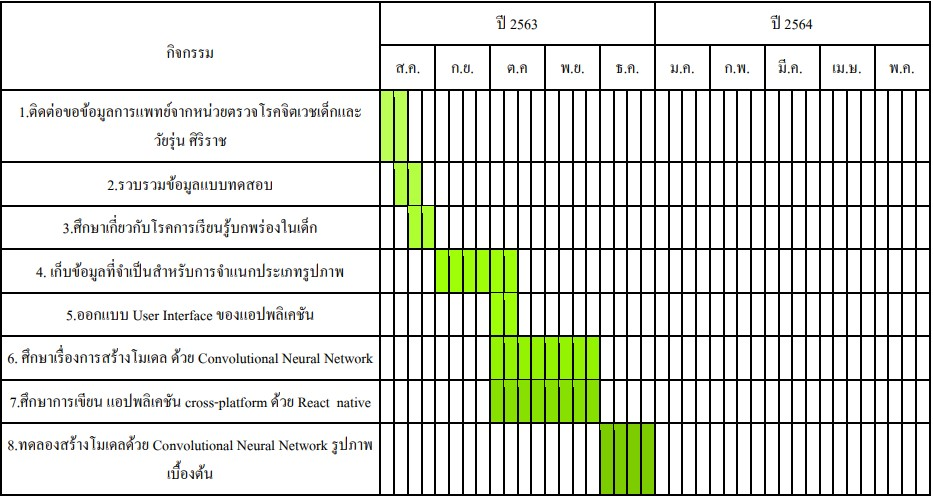
\includegraphics[height=10cm]{./gantt1.jpg}}
  \caption{ภาพตารางเวลาการทำงานภาคการศึกษาที่ 1}\label{fig:system}
 \end{figure}
 \begin{figure}[ht]\centering
  \setlength{\fboxrule}{0.2mm} % can define this in the preamble
  \setlength{\fboxsep}{1cm}
  \fbox{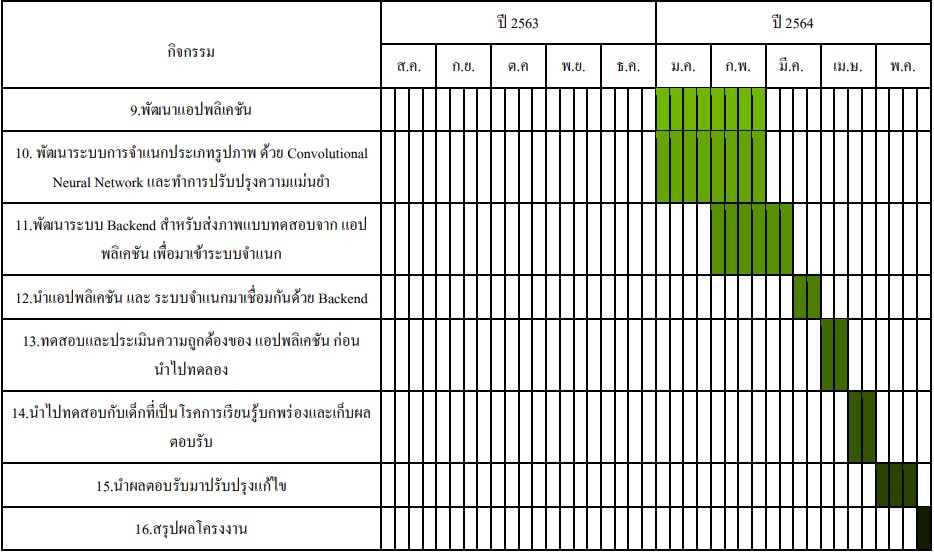
\includegraphics[height=10cm]{./gantt2.jpg}}
  \caption{ภาพตารางเวลาการทำงานภาคการศึกษาที่ 2}\label{fig:system}
 \end{figure}
\end{landscape}
\section{ผลการดำเนินงาน}
ภาคการศึกษาที่ 1 
\begin{itemize}
  \item ระบบเก็บรวบรวมข้อมูลทดสอบการเขียนของเด็กที่ได้รับบการทดสอบ
  \item ข้อมูลที่ผ่านการประมวลผลที่เตรียมพร้อมสำหรับนำไปสร้างโมเดลในการวิเคราะห์โรคบกพร่องทางการเรียนรู้
  \item โมเดลจำแนกประเภทรูปภาพแบบเบื้องต้นด้วย Convolutional Neural Network
  \item แบบจำลอง User interface ของแอปพลิเคชัน
\end{itemize}
ภาคการศึกษาที่ 2 
\begin{itemize}
  \item ระบบวิเคราะห์รูปภาพลายมือเขียนแบบทดสอบของเด็กเพื่อวินิจฉัยโอกาสเป็นโรคการเรียนรู้บกพร่องเบื้องต้นในเด็กได้อย่างแม่นยำ
  \item แอปพลิเคชัน ที่อยู่ในรูปแบบเกมส์เพื่อให้เด็กเล่นและสามารถทำแบบทดสอบไปพร้อมกันโดยจากนั้นนำภาพไปใช้ในการวินิจฉัยความเป็นไปได้ของโรคการเรียนรู้บกพร่องเบื้องต้น
  \item ผลลัพธ์ที่แม่นยำและสามารถแสดงถึงจำนวนความผิดพลาดที่เขียนผิดและความน่าจะเป็นได้
  \item ผลประเมินการใช้งานจากผู้ใช้งาน
\end{itemize}
%%%%%%%%%%%%%%%%%%%%%%%%%%%%%%%%%%%%%%%%%%%%%%%%%%%%%%%%%%%%
%%%%%%%%%%%%%%  Literature Review %%%%%%%%%%%%%%%%%%%%%%%%%%
%%%%%%%%%%%%%%%%%%%%%%%%%%%%%%%%%%%%%%%%%%%%%%%%%%%%%%%%%%%%
\chapter{ทฤษฎีความรู้และงานที่เกี่ยวข้อง}
\section{Core concept แนวคิดหลัก}
เนื่องจากตัวระบบที่เราสร้างขึ้นมาเพื่อวินิจฉัยโรคการเรียนรู้บกพร่องในเด็กนั้นจะต้องทำการเรียนรู้ข้อมูลลักษณะจุดเด่นต่างๆของภาพผลแบบทดสอบการเรียนรู้บกพร่องในเด็กว่า 
มีลักษณะเด่นใดจึงจำแนกว่าเด็กคนนั้นมีโอกาสเป็นโรคการเรียนรู้บกพร่องในเด็ก 
จากการค้นคว้าหาข้อมูลจึงพบว่าเราจำเป็นที่จะต้องใช้ความรู้ในเรื่องของ Convolutional Neural Network 
ซึ่งเหมาะแก่การทำการจำแนกประเภทของรูปภาพ และเป็นส่วนหนึ่งของเรื่องการเรียนรู้เชิงลึกของคอมพิวเตอร์ (deep learning)

\subsection{การเรียนรู้เชิงลึกของคอมพิวเตอร์ (deep learning)}

\par การเรียนรู้เชิงลึกของคอมพิวเตอร์ (deep learning) เป็นหนึ่งในสาขาย่อยของ machine learning เป็นศาสตร์ที่พูดถึงการจำลองการทำงานของระบบโครงข่ายประสาทมนุษย์ โดย จะมีการแบ่งการทำงานข้างในเป็น layer ต่างๆ โดยเราจะมองเป็นสามส่วนหลักๆได้แก่ 	

\begin{enumerate}
  \item Input Layer มีหน้าที่สำหรับการรับข้อมูลป้อนเข้าโครงข่ายประสาท จากผู้ใช้ เช่น รูปภาพ
  \item Hidden Layer มีหน้าที่สำหรับการประเมินข้อมูลที่ป้อนเข้ามา เพื่อหาข้อมูลต่างๆที่ใช้ในการจำแนกประเภทโดยตัว Hidden Layer นั้นสามารถมีได้มากกว่า 1 ชั้น
  \item Output layer เป็นชั้นสุดท้ายมีหน้าที่สำหรับรับข้อมูลจาก Hidden Layer เพื่อใช้ในการบอกว่าท้ายที่สุดแล้วตัวข้อมูลที่รับเข้ามานั้นถูกจำแนกอยู่ในประเภทใด
\end{enumerate}

\begin{figure}[!ht]\centering
  \setlength{\fboxrule}{0.2mm} % can define this in the preamble
  \setlength{\fboxsep}{1cm}
  \fbox{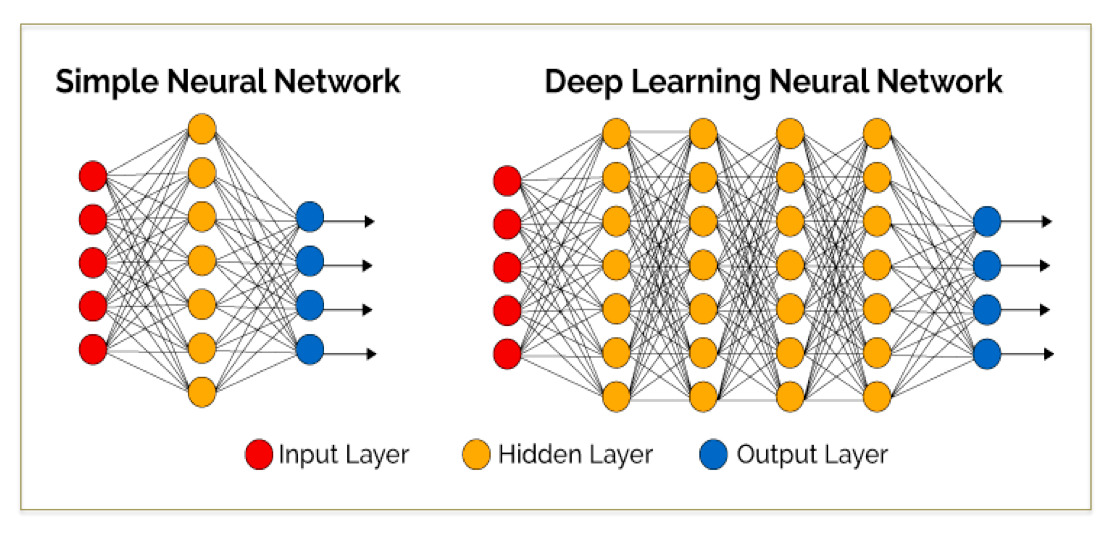
\includegraphics[width=10cm]{./DeepLearning.jpg}}
  \caption{ตัวอย่าง layer ของ การเรียนรู้เชิงลึกของคอมพิวเตอร์}\label{fig:deep}
  \source{[ที่มา : https://verneglobal.com/news/blog/deep-learning-at-scale]}
\end{figure}

\subsection{โครงข่ายประสาทเทียมแบบสังวัตนาการ (Convolutional Neural Network)\cite{CS231}} 
\FloatBarrierในปัจจุบันการทำ การจำแนกประเภทรูปภาพ สำหรับทางด้านการแพทย์กำลังเป็นที่สนใจ โครงข่ายประสาทเทียมแบบสังวัตนาการ 
หรือ CNN เลยได้รับความนิยมมากขึ้นโดย CNN เป็นรูปแบบหนึ่งของ การเรียนรู้เชิงลึกของคอมพิวเตอร์ ที่เกิดจากการนำแนวคิดของ  
Neural Network มาเพิ่มในส่วนของ Convolutional layer ซึ่งเหมาะแก่การหาลักษณะต่างๆของข้อมูลต่างๆ เช่น รูปภาพ 
โดยตัวของ CNN นั้นจะประกอบด้วยหลายๆ layer ด้วยกัน

\begin{figure}[!ht]\centering
  \setlength{\fboxrule}{0.2mm} % can define this in the preamble
  \setlength{\fboxsep}{1cm}
  \fbox{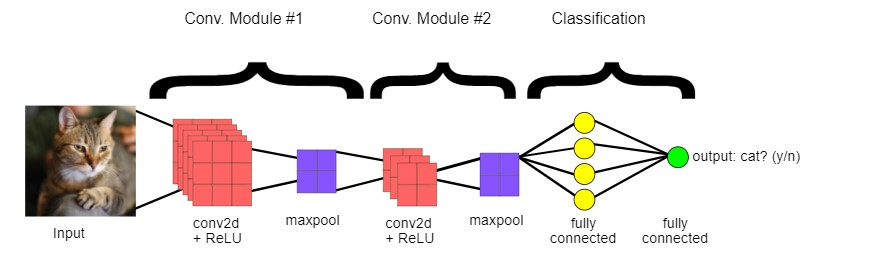
\includegraphics[width=10cm]{./cnn.jpg}}
  \caption{แสดงตัวอย่างโครงข่าย CNN ที่ประกอบด้วย 1. convolutional layer 2. pooling layer 3. fully connected layer
  }\label{fig:cnn}
  \source{[ที่มา : https://developers.google.com/machine-learning/practica/image-classification/convolutional-neural-networks]}
\end{figure}

โดย CNN จะมี layer หลักๆได้แก่ 	
\begin{enumerate}
  \item Convolutional layer ซึ่งมีหน้าที่ในการประมวลผลภาพเพื่อหาคุณลักษณะต่างๆ เช่น สี ขอบ ด้วย filters และนำไปเข้า activate function เพื่อแปลงผลลัพธ์ให้กลายเป็นข้อมูลนำเข้าสำหรับ layer ถัดไป 
  โดยมี activate function ที่ได้รับความนิยมในการทำ การจำแนกประเภทรูปภาพ คือ Rectified Linear Unit (ReLU)
  \item Pooling layer มีหน้าที่ในการลดมิติของข้อมูลที่เราได้จาก Convolutional layer ให้เล็กลง และคงไว้ซึ่งข้อมูลที่จำเป็นเพื่อที่จะทำให้การประมวลผลเร็วขึ้น โดยจะมีสองวิธีหลักๆได้แก่ 
  Max pooling และ Mean pooling โดย Max pooling จะทำการเลือกค่าที่มากที่สุดในขอบเขตที่สนใจ และ Mean Pooling จะทำการหาค่าเฉลี่ยของขอบเขตที่สนใจแล้วนำไปใช้ต่อ ดังรูป \ref{fig:pooling} 
  \begin{figure}[!ht]\centering
    \setlength{\fboxrule}{0.2mm} % can define this in the preamble
    \setlength{\fboxsep}{1cm}
    \fbox{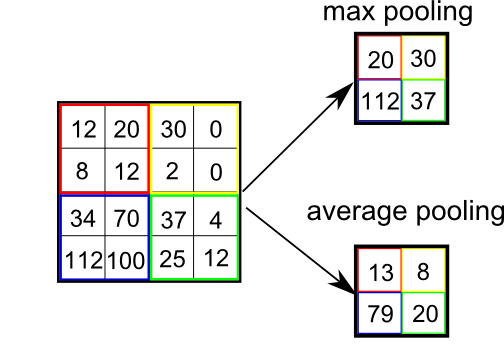
\includegraphics[width=10cm]{./pooling.png}}
    \caption{ตัวอย่างการทำ Max pooling และ mean pooling}\label{fig:pooling}
    \source{[ที่มา : https://stackoverflow.com/questions/44287965]}
  \end{figure}
  \item fully connected layer มีหน้าที่ในการรวบรวม output จาก layer ก่อนหน้า ที่ได้ทำการหา คุณลักษณะต่างๆมารวมและกำหนดให้ผลลัพธ์ของ layer นี้มีจำนวนเท่ากับ จำนวนประเภทที่เราต้องการจำแนกรูปภาพ 
  เพื่อดูว่าผลลัพธ์ท้ายสุดเราจำแนกรูปภาพนั้นได้อยู่ในประเภทไหนซึ่ง CNN จะประกอบด้วยหลายๆ layer นี้เรียงกันไปมาจนถึง output ตามความเหมาะสมของ โมเดลนั้นๆ และสามารถปรับ parameter ของแต่ละ layer ได้เพื่อทำให้การจำแนกประเภทนั้นออกมาแม่นยำที่สุด 
  โดยในโครงการนี้ เราจะเลือกใช้ Convolutional neural network ในการสร้าง โมเดลเพื่อจำแนกข้อมูลภาพถ่ายของเรา
\end{enumerate}

\subsection{Transfer Learning\cite{Transfer}}
ในการทำ Convolutional neural networkนั้น เราจำเป็นจะต้องออกแบบตัว layer และ parameter ต่างๆให้เหมาะสมเพื่อให้ได้ความแม่นยำในการจำแนกที่สูง
ซึ่งเราจำเป็นต้องใช้ข้อมูลจำนวนมากในการ train ให้โมเดล CNN ของเรานั้นมีความแม่นยำ แต่ว่า Transfer Learning คือการที่เรานำ โมเดล CNN ที่มีการสร้างขึ้นมาไว้แล้วจากข้อมูลอื่น มาปรับแต่งในส่วนของ
fully connected layer เองใหม่ให้เหมาะสมกับข้อมูลที่เราจะทำการจำแนก ซึ่งจะทำให้เราประหยัดเวลาในการสร้างโมเดล และลดจำนวนข้อมูลที่ใช้ในการสร้างโมเดลเพื่อที่จะทำให้โมเดลนั้นมีความแม่นยำ
\begin{figure}[!ht]\centering
  \setlength{\fboxrule}{0.2mm} % can define this in the preamble
  \setlength{\fboxsep}{1cm}
  \fbox{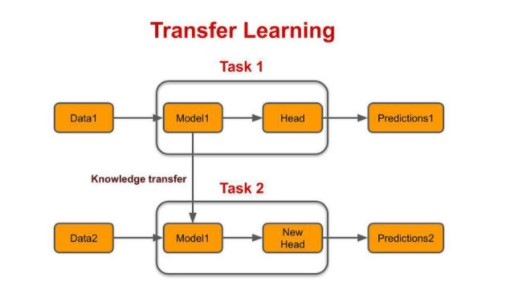
\includegraphics[width=10cm]{./transfer.jpg}}
  \caption{ภาพอธิบายตัวอย่างของ Transfer Learning}\label{fig:transfer}
  \source{[ที่มา : https://www.topbots.com/transfer-learning-in-nlp/]}
\end{figure}

\newpage 
\subsection{Activate Function\cite{Activate}}
Activate function มีหน้าที่ในการปรับผลลัพธ์ ของ neuron ในแต่ละ layer ก่อนจะส่งต่อไปเป็นข้อมูลนำเข้าสำหรับ layer ถัดไป โดย Activate function ที่เป็นที่นิยมคือ sigmoid function เนื่องจากตัว sigmoid function 
น้ันจะมีผลลัพธ์ออกมาอยู่ในช่วงของ 0 จนถึง 1 ทำให้เหมาะแก่การใช้ทำเรื่องความน่าจะเป็น แต่เนื่องจากกราฟของ sigmoid function เป็นดังรูป \ref{fig:sigmoid}  เราจะเห็นว่าหากค่า |x| มีค่าสูงมากขึ้นค่าของ sigmoid tfunction จะมีการเปลี่ยนแปลงที่น้อยลง 
หรือมีค่าอนุพันธ์ที่น้อยลงทำให้การอัพเดทน้ำหนักของตัว Neural network ใน layer แรกๆนั้นมีค่าน้อยจนอาจทำให้การเรียนรู้หยุด  
ปัญหานี้มีชื่อเรียกว่า Vanishing gradient problem โดยสามารถแก้ไขด้วยการเปลี่ยน activate function ได้ยกตัวอย่างเช่น Rectified Linear Unit หรือ ReLU

\begin{figure}[!ht]\centering
  \setlength{\fboxrule}{0.2mm} % can define this in the preamble
  \setlength{\fboxsep}{1cm}
  \fbox{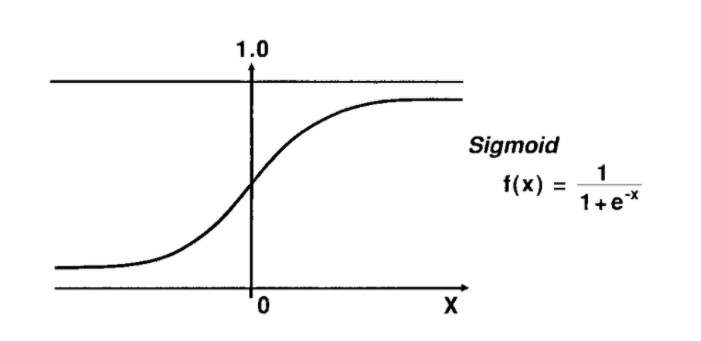
\includegraphics[width=10cm]{./sigmoid.jpg}}
  \caption{ภาพตัวอย่างกราฟของ sigmoid function}\label{fig:sigmoid}
  \source{[ที่มา : https://www.researchgate.net/figure/An-illustration-of-the-signal-processing-in-a-sigmoid-function_fig2_239269767]}
\end{figure}

\subsection{Rectified Linear Unit (ReLU)\cite{ReLuFunc}}
Rectified Linear Unit หรือ ReLU เป็น activate function ที่กำลังได้รับความนิยมเนื่องจากสามารถแก้ไขปัญหาในเรื่องของ 
anishing gradient problem ได้ เพราะกราฟของ ReLU นั้นถ้าค่า x เป็นบวกจะได้ค่าของอนุพันธ์เท่ากับ 1 เสมอทำให้ความชันไม่หาย 
ซึ่งทำให้ตัวโมเดลของเรานั้นปรับค่าน้ำหนักได้ไวยิ่งขึ้น แต่ก็มีข้อเสียเช่นกันคือผลลัพธ์จะออกมาอยู่ในช่วงตั้งแต่ 0 ถึง อินฟินิตี้ทำให้ไม่สามารถกำหนดขอบเขตได้ หรือผลลัพธ์สำหรับการที่ข้อมูลขาเข้าเป็นเลขติดลบจะเท่ากับ 
0 เสมอทำให้ไม่สามารถแปลงค่าผลลัพธ์ที่เท่ากับ 0 กลับมาเป็นข้อมูลขาเข้าได้ เป็นต้น 


\begin{figure}[!ht]\centering
  \setlength{\fboxrule}{0.2mm} % can define this in the preamble
  \setlength{\fboxsep}{1cm}
  \fbox{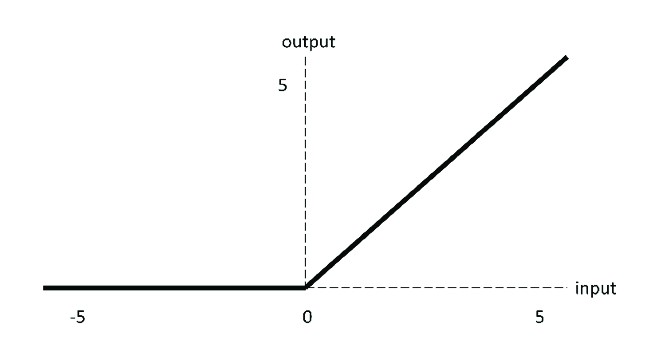
\includegraphics[width=5cm,height=3cm]{./relu.jpg}}
  \caption{ภาพตัวอย่างกราฟของ ReLU function}\label{fig:relu}
  \source{[ที่มา : https://www.researchgate.net/figure/ReLU-activation-function_fig7_333411007]}
\end{figure}



\subsection{การปรับขนาดรูปภาพ (Image rescale)\cite{Imagepre}}
การปรับขนาดรูปภาพ (Image rescale) นั้นเป็นส่วนหนึ่งของกระบวนการเตรียมข้อมูลเบื้องต้นสำหรับการทำโมเดล CNN 
เนื่องมาจากข้อมูลที่เราได้มาสำหรับการทำโมเดลนั้น อาจจะมีขนาดที่แตกต่างกันรวมถึงมีขนาดที่ใหญ่เกินไป ด้วยเหตุนั้นจะทำให้โมเดลใช้ระยะเวลาในการเรียนรู้นาน 
เราจึงกำหนดขนาดมาตรฐานและทำการปรับขนาดข้อมูลรูปภาพสำหรับการสร้างโมเดลก่อนที่จะนำไปใช้

\subsection{การแยกบริเวณรูปภาพ (Image segmentation)\cite{Imagesegment}}
การแยกบริเวณรูปภาพ (Image segmentation) คือการแยกสิ่งที่เราสนใจออกมาจากพื้นหลังของรูปภาพเพื่อใช้ในการทำโมเดลต่อไป ซึ่งถูกนำไปใช้ประโยชน์ในหลายๆด้านด้วยกันได้แก่ 
การจับตัวหนังสือในภาพ การจับวัตถุแปลกปลอมในรูปภาพเป็นต้น โดยมีหลายรูปแบบด้วยกันยกตัวอย่างเช่น Region-Based Segmetation, Edge Detection Segmentation เป็นต้น
\begin{itemize}
  \item Region-Based Segmentation เป็นการแยกวัตถุออกจากภาพด้วยวิธีการใช้ค่า threshold เพื่อปรับภาพที่อยู่ในรูปแบบของ grayscale ให้กลายเป็น binary image โดยให้วัตถุเป็นหนึ่งสี และ พื้นหลังเป็นอีกสีหนึ่ง เพื่อที่เราจะได้รูปร่างของวัตถุขึ้นมา ซึ่งวิธีการเลือกค่า threshold ที่เหมาะสมมีมากมาย ยกตัยวอย่างเช่น Otsu’s thresholdig method

  \item Edge Detection Segmentation ที่ใช้ในการหาขอบของวัตถุซึ่งใช้หลักการความไม่ต่อเนื่องภายใน pixel ของรูปภาพ โดยจุดที่เกิดการเปลี่ยนแปลงนั้นจะถูกระบุเป็นจุดขอบ 
  \item Output layer เป็นชั้นสุดท้ายมีหน้าที่สำหรับรับข้อมูลจาก Hidden Layer เพื่อใช้ในการบอกว่าท้ายที่สุดแล้วตัวข้อมูลที่รับเข้ามานั้นถูกจำแนกอยู่ในประเภทใด
\end{itemize}
\begin{figure}[!ht]\centering
  \setlength{\fboxrule}{0.2mm} % can define this in the preamble
  \setlength{\fboxsep}{1cm}
  \fbox{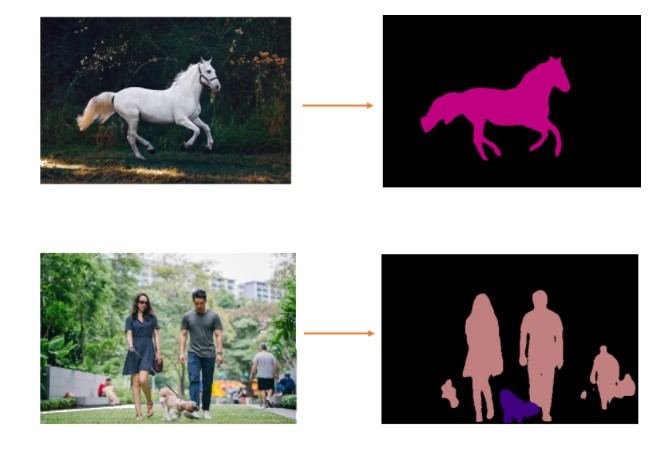
\includegraphics[width=10cm]{./imagesegment.jpg}}
  \caption{ภาพตัวอย่างการทำ image segmentation บนภาพ}\label{fig:imagesegment}
  \source{[ที่มา : https://www.learnopencv.com/applications-of-foreground-background-separation-with-semantic-segmentation/]}
\end{figure}


\newpage
\subsection{การแปลงรูปภาพเป็นข้อความ (Optical character recognition)}
Optical character recognition หรือ OCR คือเทคโนโลยีที่ทำให้เราสามารถจับตัวอักษรที่อยู่ในภาพถ่ายยกตัวอย่างเช่น ภาพสแกนของเอกสาร หรือ สื่อสิ่งพิมพ์ต่างๆเป็นต้น มาแปลงให้อยู่ในรูปแบบของตัวอักษรดิจิตอล
 ที่สามารถแก้ไขได้ และง่ายต่อการจัดเก็บนำไปใช้ต่อ ซึ่งเราสามารถนำเทคโนโลยีไปประยุกต์ใช้ได้ในหลากหลายด้าน เช่น วิเคราะห์ทะเบียนรถยนต์ ด้านการทำระบบค้นหาข้อมูล หรือระบบจัดเก็บรายละเอียดสินค้า

\begin{figure}[!ht]\centering
  \setlength{\fboxrule}{0.2mm} % can define this in the preamble
  \setlength{\fboxsep}{1cm}
  \fbox{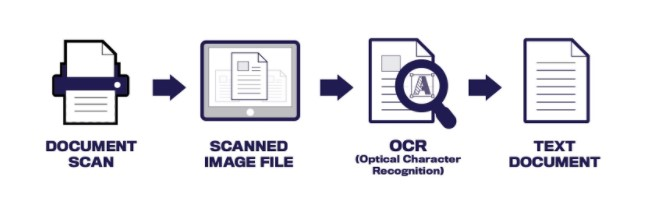
\includegraphics[width=10cm]{./ocr.jpg}}
  \caption{ภาพตัวอย่างขั้นตอนการแปลงเอกสารมาอยู่ในรูปแบบข้อมูลด้วยกระบวนการ OCR}\label{fig:ocr}
  \source{[ที่มา : https://medium.com/states-title/using-nlp-bert-to-improve-ocr-accuracy-385c98ae174c]}
\end{figure}

\subsection{Blob coloring}
ใช้ในการทำ OCR ของเราเป็นอัลกอริทึมที่ใช้ในการแบ่งขอบเขตของวัตถุ โดยจะทำการไล่ตั้งแต่ pixel บนสุดของภาพลงมาล่างสุดซึ่งแต่ละ
 pixel จะทำการจับว่า pixel รอบๆตัวนั้นเป็นสีดำหรือไม่ หากเป็นสีดำก็จะจับให้ pixel เหล่านั้นอยู่ใน label เดียวกัน ซึ่งวิธีการนี้จะทำให้เราสามารถแยกตัวอักษรแต่ละตัวออกจากกันได้ โดยแต่ละตัวก็จะมี label ของตัวมันเอง

\begin{figure}[!ht]\centering
  \setlength{\fboxrule}{0.2mm} % can define this in the preamble
  \setlength{\fboxsep}{1cm}
  \fbox{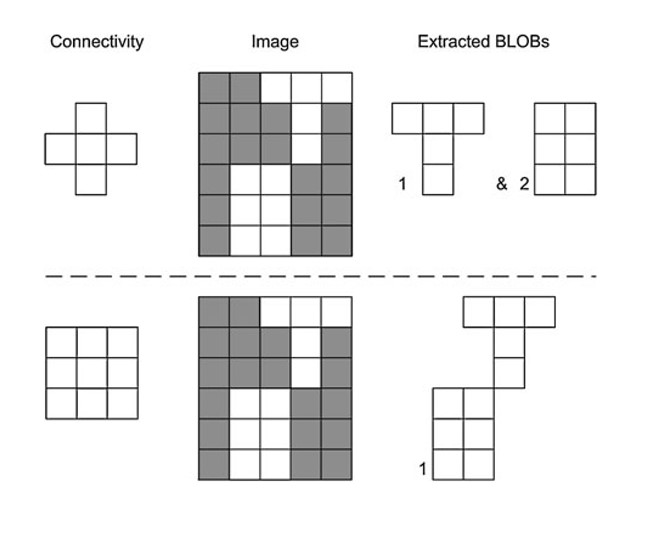
\includegraphics[width=8cm,height=5cm]{./blob.jpg}}
  \caption{ภาพตัวอย่างการทำงานของ Blob coloring}\label{fig:blob}
  \source{[ที่มา : http://what-when-how.com/introduction-to-video-and-image-processing/blob-analysis-introduction-to-video-and-image-processing-part-1/]}
\end{figure}



\section{Languages and technologies  ภาษาโปรแกรมและเทคโนโลยี}
เนื่องด้วยด้วยเป้าหมายของโครงการที่่ต้องการพัฒนาแอปพลิเคชันให้สามารถใช้งานได้ในหลายแพลตฟอร์ม 
โดยปัจจุบันระบบปฎิบัติการแอนดรอยด์และระบบปฎิบัติการไอโอเอสเป็นระบบปฎิบัติการที่ผู้คนใช้งานมากที่สุด 
โดยทั้งสองระบบปฎิบัติการครอบครองส่วนแบ่งทางตลาดมากกว่า 98\%  สำหรับโทรศัพท์มือถือและแท็ปเล็ต
\begin{figure}[!ht]\centering
  \setlength{\fboxrule}{0.2mm} % can define this in the preamble
  \setlength{\fboxsep}{1cm}
  \fbox{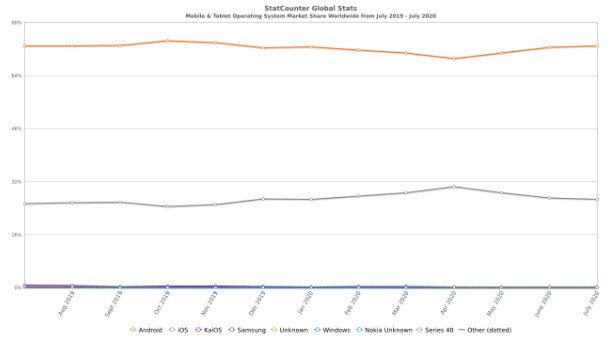
\includegraphics[width=10cm]{./market.jpg}}
  \caption{ส่วนแบ่งการตลาดระบบปฏิบัติการมือถือและแท็บเล็ตทั่วโลก}\label{fig:market}
  \source{[ที่มา : https://gs.statcounter.com/os-market-share/mobile-tablet/worldwide/#monthly-201907-202007]}
\end{figure}
จากสถิติระบบปฎิบัติการไอโอเอสและระบบปฎิบัติการแอนดรอยด์มีจำนวนผู้ใช้ปริมาณมาก ดังนั้นโครงการจึงพัฒนาแอปพลิเคชันให้สามารถใช้งานได้ทั้งสองระบบปฎิบัติการ 
ซึ่งรูปแบบในการพัฒนาแอปพลิเคชันให้สามารถใช้งานในหลายแพลตฟอร์มได้มีด้วยกันอยู่สองรูปแบบคือ Hybrid Application และ Web Application อย่างไรก็ตาม Hybrid Application 
สามารถทำงานได้ตามเป้าหมายของโครงการมากกว่าเพราะการเป็นรูปแบบแอปพลิเคชันทำให้สามารถใช้หน้าจอสัมผัสผ่านโทรศัพท์มือถือหรือแท็บเล็ตในการเขียนตัวอักษรได้ โดยมีเฟรมเวิร์คให้พัฒนามากมายเช่น React Native ,Ionic และ Flutter เป็นต้น


\subsection{React Native}
React Native คือ เฟรมเวิร์คที่พัฒนาด้วยภาษา JavaScript สำหรับการพัฒนาแอปพลิเคชันสำหรับระบบปฎิบัติการไอโอเอสและระบบปฎิบัติการแอนดรอยด์โดยใช้เทคโนโลยี 
Cross platform ซึ่งในการพัฒนาด้วย React Native มีข้อดีคือในการพัฒนาสามารถพัฒนาแค่ครั้งเดียวแต่สามารถใช้งานได้ทั้งระบบปฎิบัติการไอโอเอสและระบบปฎิบัติการแอนดรอยด์ 
ด้วยการจัดการของ JavaScript ให้สามารถสื่อสารกับฝั่ง Native ของระบบปฎิบัติการทั้งสอง จึงได้ผลลัพธ์ออกมาเป็น Native Application ทั้งระบบปฎิบัติการไอโอเอสและระบบปฎิบัติการแอนดรอยด์ 

\subsection{Keras}
Keras คือเฟรมเวิร์คที่พัฒนาด้วยภาษา Python ที่ถูกสร้างขึ้นมาเพื่อให้เราสามารถจัดการกับการทำ การเรียนรู้เชิงลึกของคอมพิวเตอร์ (deep learning) 
ได้อย่างง่าย ข้อดีของ Keras คือ ใช้งานง่าย และสามารถดัดแปลงตัว layer ของ neural network ได้ง่าย  โดยในโครงการนี้เราสามารถใช้ Keras 
ในการออกแบบตัว Layer ต่างๆ ของโมเดลได้รวมทั้งทำการสร้างโมเดลและทำนายด้วยภาษา Python ได้เลย

\subsection{OpenCV\cite{OpenCV}}
OpenCV เป็น library ที่มีจุดประสงค์เพื่อการแสดงผลด้วยคอมพิวเตอร์แบบเรียลไทม์  (Real - Time) รวมทั้งในส่วนของการทำ Image processing ที่รองรับการใช้งานบนหลายภาษาด้วยกัน
 โดยหนึ่งในนั้นคือ Python อีกทั้งยังสามารถใช้งานร่วมกับเฟรมเวิร์กการเรียนรู้เชิงลึกต่างๆ อาทิเช่น TensorFlow และ PyTorch  เป็นต้น 

\subsection{Django Rest Framework}
Django Rest Framework เป็น framework ที่พัฒนาขึ้นมาด้วยภาษา python ไว้ใช้สำหรับการสร้าง api ไว้คุยกับฐานข้อมูล  
เพื่อให้ website หรือ application สามารถเรียกใช้ตัว api เพื่อขอข้อมูล  ซึ่งสามารถพัฒนาได้ง่ายด้วยภาษา python
และที่เราเลือกเนื่องจากตัวโมเดลวินิจฉัยโรคของเราก็พัฒนาขึ้นจากภาษา python เช่นเดียวกันทำให้สามารถเรียกใช้งานได้ง่าย

\section{Related research / Competing solutions บทความที่เกี่ยวข้อง}

\subsection{Detecting Dyslexia Using Neural Networks\cite{Dyslexia}}
\begin{figure}[!ht]\centering
  \setlength{\fboxrule}{0.2mm} % can define this in the preamble
  \setlength{\fboxsep}{1cm}
  \fbox{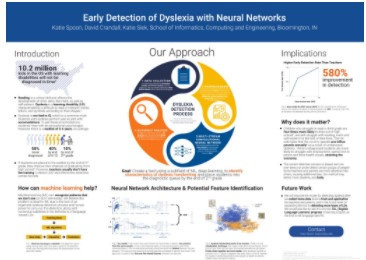
\includegraphics[width=6cm,height=5cm]{./dyslexia.jpg}}
\end{figure}

\subsubsection{การใช้ภาพลายมือในการวินิจฉัยโรค Dyslexia}
มีงานจำนวนมากที่วินิจฉัยโรค Dyslexia โดยการใช้ข้อมูลคะแนนการสอบ ประวัติของผู้ทดสอบ หรือ แบบสอบถาม และมีอีกจำนวนหนึ่งที่ใช้ข้อมูลเช่นภาพการทำงานของสมอง หรือ การสื่อสารผ่านทางดวงตาเป็นต้น 
แต่วรรณกรรมนี้ได้เลือกที่จะใช้ข้อมูลลายมือเนื่องจาก เป็นข้อมูลที่ง่ายต่อการเก็บรวบรวม


\subsubsection{การประมวลผลภาพ}
ในส่วนของการประมวลผลภาพนั้น วรรณกรรมนี้ได้ทำการนำภาพลายมือมาแบ่งเป็นบรรทัด 
หลังจากนั้นจึงได้นำแต่ละบรรทัดมาแบ่งเป็นอีก 50 ส่วน โดยวิธีการที่ใช้ในการแบ่งบรรทัด คือ 
 Arvanitopoulos & Susstrunk’s seam carving แล้วจึงนำภาพแต่ละบรรทัดไปแบ่งเป็น 50 
 ส่วนโดยใช้ขนาด 113*113 ซึ่งยังมีบางภาพที่ยากต่อการทำ แล้วจำเป็นต้องใช้การแก้ไขโดยผู้จัดทำก่อน แต่ไม่ได้มีความยากในการแก้ไขสูง

 \subsubsection{Optical character recognition}
 Optical character recognition หรือ OCR นั้นเป็นการจับตัวอักษรภายในภาพแล้วจึงนำมาแปลงเป็นค่า
  วิธีนี้สามารถอ่านได้ว่าในภาพนั้นมีตัวอักษรตัวใดอยู่บ้าง แต่จากการทดลองของวรรณกรรมนี้พบว่า 
  วิธีนี้ไม่เหมาะสมกับการนำมาอ่านภาพลายมือของเด็กที่เป็นโรค 
  เนื่องจากลายมือของเด็กนั้นมีความหลากหลายมาก ทำให้วิธีการตรวจจับด้วยระบบ OCR ไม่สามารถตรวจจับได้อย่างแม่นยำ
\subsubsection{การทำโมเดลวินิจฉัย}
เป็นส่วนที่ให้โมเดลนั้นได้ทำการระบุว่าข้อมูลที่ป้อนเข้ามาเป็นโรค dyslexia หรือไม่ 
โดยตัวโมเดลนั้นอยู่ในรูปแบบของ  โครงข่ายประสาทเทียมแบบสังวัตนาการ 
หรือ Convolutional Neural Network โดยประกอบด้วย convolutional layer จำนวน 5 layer 
max-pooling จำนวน 3 layer fully-connected จำนวน 2 layer และ dropout layer จำนวน 1 layer 
หลังจากนั้นจึงได้แบ่งข้อมูลแบบ 3:1:1 โดยเป็นข้อมูลในส่วนของการ train 60% test 20% และ validation 20% และได้ทดลองทำการเรียนรู้โมเดลด้วย batch size และจำนวนส่วนของแถวที่แบ่ง ด้วยหลายๆค่า โดยได้ค่าที่เหมาะสมคือ batch size = 4 และ แบ่ง 50 ส่วนต่อแถวของคำพูด

วรรณกรรมนี้ เป็นวรรณกรรมที่ดีและมีคล้ายกับว่ามีข้อเสนอแนะว่าไม่ควรใช้อะไรบ้าง 
รวมถึงช่วยเรื่องการคิดระบบการทำงานว่าควรมีขั้นตอนแบบใดจากวิธีแรกถึงวิธีสุดท้าย
 เห็นได้ว่ามีหลายวิธีอยากมากที่วินิจฉัยเรื่องของการเป็น LD แต่ว่าโปรเจ็คของเขาได้เลือกวิธีการวินิจฉัย
 ผ่านลายมือเนื่องจากสามารถเก็บรวบรวมได้ง่าย หลังจากนั้นนำภาพมาแบ่งเป็น 50 ส่วนตามขนาด 113*113 
 แต่ก็พบว่ายังมีบางภาพที่สามารถตัดแบ่งได้ยาก และใช้ OCR ในการระบุด้วย ผลออกมาคือมาความแม่นยำที่น้อย







%%%%%%%%%%%%%%%%%%%%%%%%%%%%%%%%%%%%%%%%%%%%%%%%%%%%%55
%%%%%%%%%%%%%%%%%%%%%%%%%%%%%%%%%%%%%%%%%%%%%%%%%%%%%
%%%%%%%%%%%%%%%%%%%%%%%%%%%%%%%%%%%%%%%%%%%%%%%%%%%%%
\chapter{วิธีการดำเนินงาน}
ในส่วนของวิธีการดำเนินงานจะกล่าวถึงขั้นตอนการวางแผนงานและระบบงานต่างๆของแอปพลิเคชัน LDSpot โดยจะประกอบด้วยหัวข้อต่างๆ ได้แก่ System Architecture, System Requirement, Process flow, Use cases, โครงสร้างซอฟต์แวร์, Conceptual Design, Database Design, Sequence Diagram Design, User Interface Design และการเก็บภาพลายมือเด็ก
\section{Project Functionality}
\subsection{System Architecture}
\begin{figure}[!ht]\centering
  \setlength{\fboxrule}{0.2mm} % can define this in the preamble
  \setlength{\fboxsep}{1cm}
  \fbox{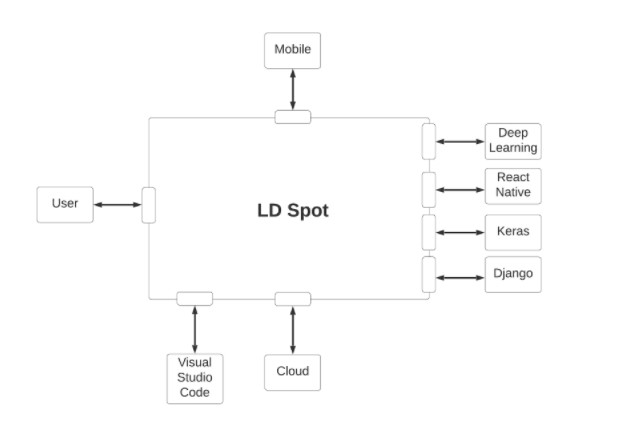
\includegraphics[width=10cm]{./system.jpg}}
  \caption{ภาพ System Architecture ของ LDSpot}\label{fig:system}
\end{figure}
\subsection{System requirements}
\begin{itemize}
  \item รองรับระบบปฏิบัติการแอนดรอยด์ตั้งแต่ 4.1 ขึ้นไป
  \item รองรับระบบปฏิบัติการไอโอเอสตั้งแต่ 10.0 ขึ้นไป
  \item รองรับระบบสัมผัสหน้าจอ
  \item สามารถดูผลการวินิจฉัยย้อนหลังได้
  \item อนุญาติให้เก็บผลการวินิจฉัยบนระบบได้
\end{itemize}
\newpage
\subsection{Process Flow}
\begin{figure}[!ht]\centering
  \setlength{\fboxrule}{0.2mm} % can define this in the preamble
  \setlength{\fboxsep}{1cm}
  \fbox{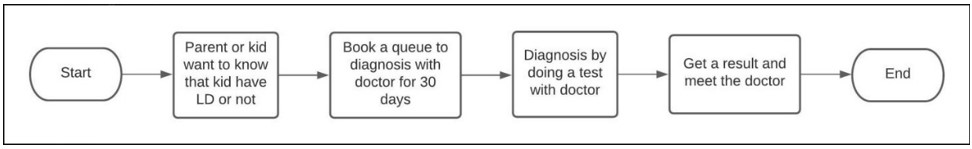
\includegraphics[width=14cm]{./processflowbefore.jpg}}
  \caption{ภาพขั้นการทำงานของบุคลากรทางการแพทย์ก่อนใช้แอปพลิเคชัน LDSpot}\label{fig:usecase}
\end{figure}
\begin{figure}[!ht]\centering
  \setlength{\fboxrule}{0.2mm} % can define this in the preamble
  \setlength{\fboxsep}{1cm}
  \fbox{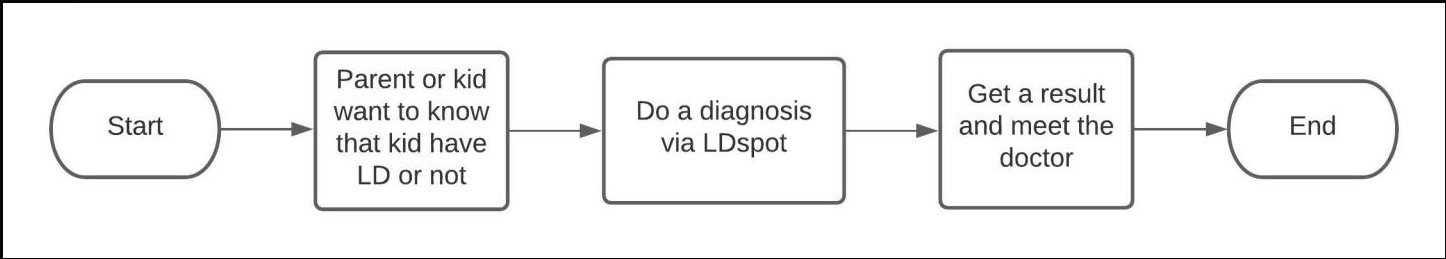
\includegraphics[width=14cm]{./processflowafter.jpg}}
  \caption{ภาพขั้นตอนการทำงานของบุคลากรทางการแพทย์หลังใช้แอปพลิเคชัน LDSpot}\label{fig:usecase}
\end{figure}
\newpage
\subsection{Use cases}
\begin{figure}[!ht]\centering
  \setlength{\fboxrule}{0.2mm} % can define this in the preamble
  \setlength{\fboxsep}{1cm}
  \fbox{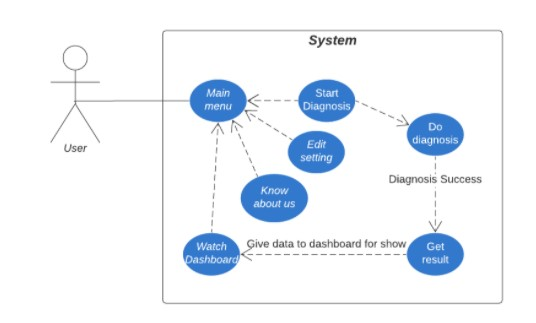
\includegraphics[]{./usecase.jpg}}
  \caption{ภาพ Use Case Diagram}\label{fig:usecase}
\end{figure}
เมื่อผู้ใช้เข้าสู่แอปพลิเคชันของเราสิ่งแรกที่พบคือ หน้าหลัก (Main menu) เพื่อที่สามารถเชื่อมหรือใช้ฟังค์ชั่นอื่น ๆ โดยมี 4 ฟังค์ชั่น อย่างแรกเลย 
การวินิฉัย(Start Diagnosis) เมื่อผู้ใช้เลือกใช้ฟังค์ชั่นนี้ ทำให้เริ่มการวินิจฉัยโดยมีลักษณะคล้ายเกมส์ ให้เขียนตัวอักษร สระ และสะกดคำ จนเสร็จสมบูรณ์จากนั้น ก็วิเคราะห์ออกมาจากคำตอบที่เด็กได้ตอบระหว่างเกมส์ 
เพื่อให้ได้ผลลัพท์รวมถึง ส่งผลลัพธ์นั้นไปบอร์ดสถิติ (Dashboard) เพื่อที่แสดงข้อมูลให้ผู้ใช้คนอื่น ๆ เห็น นอกจากนี้ยังมีหน้าตั้งค่า(Setting) หน้าเกี่ยวกับเรา (About us) 

\section{โครงสร้างซอฟต์แวร์}
ในส่วนของการใช้งานระบบ LDSpot นั้นจะแบ่งเป็นสี่ส่วนหลักๆได้แก่ แอปพลิเคชันทำแบบทดสอบ การประมวลผลภาพ การแยกภาพ การวินิจฉัย โดยมีขั้นตอนของตัวระบบดังนี้
\begin{enumerate}
  \item ผู้ใช้จะต้องทำแบบทดสอบภายในแอปพลิเคชันโดยจะอยู่ในรูปแบบของเกมเขียน พยัญชนะ สระ และ สะกดคำ
  \item หลังจากนั้นภาพแบบทดสอบที่ผู้ใช้ได้ทำจะถูกส่งเข้าไปภายในระบบ LDSpot เพื่อทำการปรับปรุงคุณภาพของรูปภาพได้แก่การปรับขนาดของภาพให้เหมาะสม การลดสัญญาณรบกวนในภาพ และการปรับสีให้อยู่ในรูปแบบของขาวดำ
  \item เมื่อได้ภาพที่ผ่านการทำการปรับปรุงคุณภาพของภาพแล้ว ภาพจะถูกนำมาแบ่งเป็นช่องตามตัวอักษรโดยการสร้าง contour แล้วตีกรอบด้วย boundingbox ล้อมรอบแต่ละตัวอักษร หลังจากนั้นจึงตัดภาพตาม boundingbox ที่ได้สร้างไว้
  \item นำภาพแต่ละตัวอักษรเข้าไปวินิจฉัย เพื่อนำผลลัพธ์จากโมเดลมาแสดงผลบนแอปพลิเคชัน
\end{enumerate}

\end{itemize}
\newpage
\begin{figure}[!ht]\centering
  \setlength{\fboxrule}{0.2mm} % can define this in the preamble
  \setlength{\fboxsep}{1cm}
  \fbox{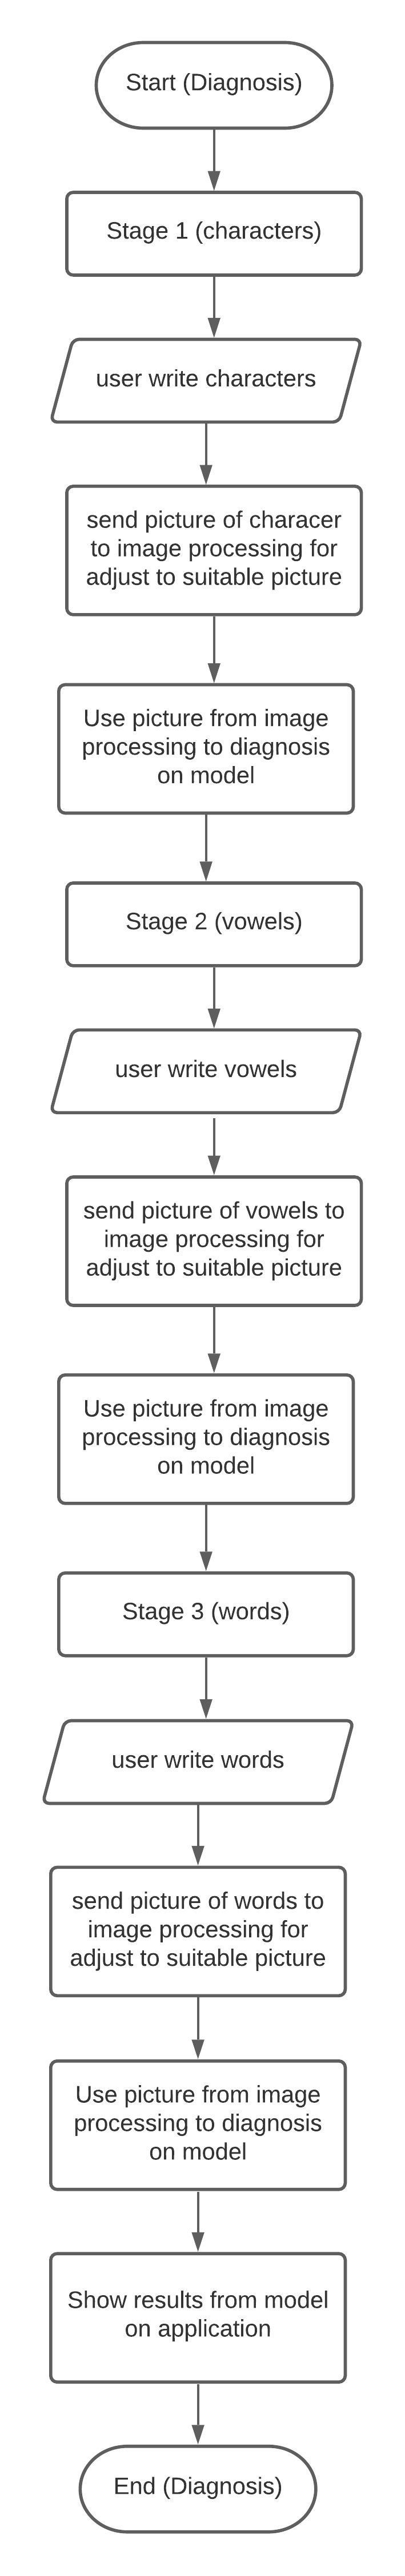
\includegraphics[scale=0.5]{./fcProcessLDsenior.jpeg}}
  \caption{ภาพ Activity diagram การดูข้อมูลสถิติในแอปพลิเคชัน}\label{fig:activity3}
 \end{figure}
 \newpage
\subsection{แอปพลิเคชันทำแบบทดสอบ (Application)}
ในส่วนของแอปพลิเคชันทำแบบทดสอบนั้นเพื่อที่จะได้มาซึ่งภาพแบบทดสอบเราจึงออกแบบแอปพลิเคชันส์ในรูปแบบของเกมให้ผู้ใช้ทำ ซึ่งในส่วนนี้ผู้ใช้จะต้องทำแบบทดสอบการเขียนพยัญชนะ สระ และสะกดคำ โดยจะมีกรอบขึ้นมาให้ผู้ใช้เขียนตามเสียงพูด 
\begin{table}[!h]\centering
  \caption{แสดงข้อมูลขาเข้าและขาออกของ แอปพลิเคชัน}\label{tbl:application1}
  \begin{tabular}{c|c|l|rr} \hline
  Input & ผู้ใช้ทำแบบทดสอบภายในแอปพลิเคชัน \\ \hline
  Output & ภาพแบบทดสอบการเขียนพยัญชนะ สระ และ คำสะกด \\ \hline
  \end{tabular}
  \end{table}

\subsection{การประมวลผลภาพ (Image processing)}
ในส่วนนี้นั้นเราจะนำภาพแบบทดสอบที่ได้จากแอปพลิเคชันมาปรับปรุงคุณภาพของภาพเพื่อให้เหมาะสมแก่การนำไปวินิจฉัย 
โดยจะมีการปรับขนาดของภาพให้ตรงกับขนาดของภาพที่ระบบ LDSpot นั้นใช้ในการเรียนรู้ หลังจากนั้นจึงนำภาพไปทำการลดสัญญาณรบกวนด้วยวิธีการใช้ 
Gaussian blur และจึงปรับภาพให้อยู่ในสีขาวดำ เพื่อแยกตัวอักษรออกจากภาพพื้นหลัง
\begin{figure}[!ht]\centering
  \setlength{\fboxrule}{0.2mm} % can define this in the preamble
  \setlength{\fboxsep}{1cm}
  \fbox{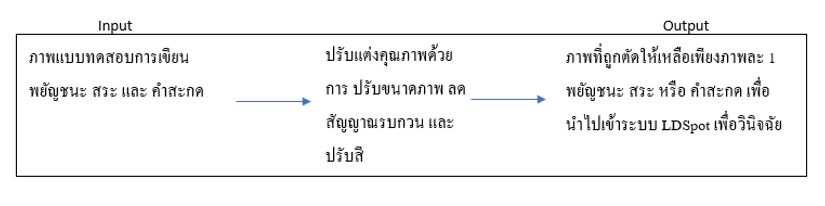
\includegraphics[width=12cm]{./imageprocess.jpg}}
  \caption{แผนภาพแสดงข้อมูลขาเข้าและออกของการประมวลผลภาพ}\label{fig:system}
\end{figure}
\begin{table}[!h]\centering
  \caption{แสดงข้อมูลขาเข้าและขาออกของส่วนการประมวลผลภาพ}\label{tbl:application1}
  \begin{tabular}{c|c|l|rr} \hline
  Input & ภาพแบบทดสอบการเขียนพยัญชนะ สระ และ คำสะกด \\ \hline
  Output & ภาพแบบทดสอบการเขียนพยัญชนะ สระ และ คำสะกดที่ปรับปรุงคุณภาพสำหรับการทำโมเดลแล้ว \\ \hline
  \end{tabular}
  \end{table}
  

  \subsection{การแยกภาพ (Image segmentation)}
  ในส่วนนี้เราจะทำการสร้าง contour ขึ้นมาจากภาพที่ได้ทำการปรับสีขาวดำแล้ว โดยเราจะนำ contour นั้นไปสร้าง bounding box
   เพื่อครอบแต่ละตัวอักษรให้แยกออกจากกัน เนื่องจากเราต้องการภาพตัวอักษรที่อยู่เดี่ยวๆ ไปใช้ในการวินิจฉัยโรคบกพร่องทางการเรียนรู้ 
  \begin{figure}[!ht]\centering
    \setlength{\fboxrule}{0.2mm} % can define this in the preamble
    \setlength{\fboxsep}{1cm}
    \fbox{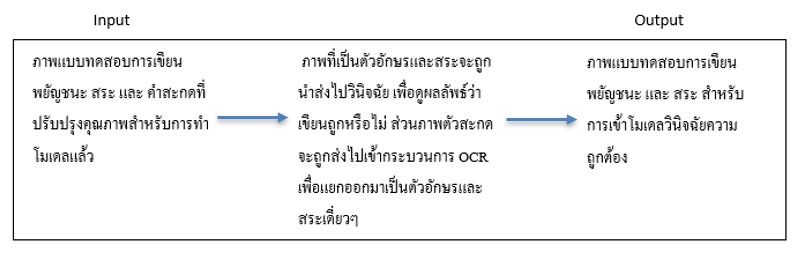
\includegraphics[width=12cm]{./imagesegment3.jpg}}
    \caption{แผนภาพแสดงข้อมูลขาเข้าและออกของการแยกภาพ}\label{fig:system}
   \end{figure}
  \begin{table}[!h]\centering
    \caption{แสดงข้อมูลขาเข้าและขาออกของส่วนการแยกภาพ}\label{tbl:application1}
    \begin{tabular}{c|c|l|rr} \hline
    Input & ภาพแบบทดสอบการเขียนพยัญชนะ สระ และ คำสะกดที่ปรับปรุงคุณภาพสำหรับการทำโมเดลแล้ว  \\ \hline
    Output & ภาพที่ถูกตัดให้เหลือเพียงภาพละ 1 พยัญชนะ สระ หรือ คำสะกด เพื่อนำไปเข้าระบบ LDSpot เพื่อวินิจฉัย\\ \hline
    \end{tabular}
    \end{table}

  \newpage
  \subsection{การวินิจฉัย (Learning disorder prediction)}
  เมื่อเราได้ภาพตัวอักษรเดี่ยวๆจากส่วนการแยกภาพแล้ว เราจะนำภาพตัวอักษรเดี่ยวๆนั้นไปโยนเข้าโมเดลที่เราได้ทำการสร้างไว้ 
  เพื่อให้โมเดลวินิจฉัยโรคบกพร่องทางการเรียนรู้ แล้วนำผลลัพธ์ส่งกลับไปในฐานข้อมูลเพื่อให้แอปพลิเคชันสามารถเรียกข้อมูลไปแสดงได้ต่อไป 
  \begin{figure}[!ht]\centering
    \setlength{\fboxrule}{0.2mm} % can define this in the preamble
    \setlength{\fboxsep}{1cm}
    \fbox{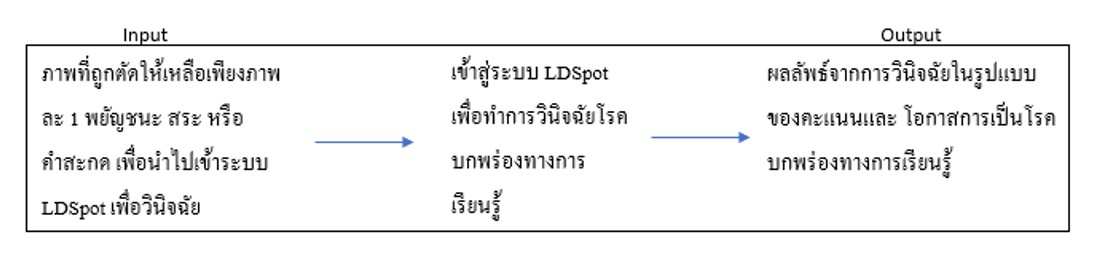
\includegraphics[width=12cm]{./imagepredict3.jpg}}
    \caption{แผนภาพแสดงข้อมูลขาเข้าและออกของการวินิจฉัย}\label{fig:system}
   \end{figure}
  \begin{table}[!h]\centering
    \caption{แสดงข้อมูลขาเข้าและขาออกของส่วนการวินิจฉัย}\label{tbl:application1}
    \begin{tabular}{c|c|l|rr} \hline
    Input & ภาพที่ถูกตัดให้เหลือเพียง ภาพละ 1 พยัญชนะ สระ หรือ คำสะกด เพื่อนำไปเข้าระบบ LDSpot เพื่อวินิจฉัย  \\ \hline
    Output & ผลลัพธ์จากการวินิจฉัยในรูปแบบของคะแนนและ โอกาสการเป็นโรคบกพร่องทางการเรียนรู้ \\ \hline
    \end{tabular}
    \end{table}
 \subsection{การหาลำดับตัวอักษรเพื่อทำนายคำสะกด (OCR}
  กรณีเฉพาะสำหรับคำสะกดเราจะนำภาพที่เด็กได้ทำการเขียนมาเข้า OCR เพื่อหาว่าการเรียงของตัวอักษรที่เด็กเขียนตรงกับคำสะกดนั้นหรือไม่ เพื่อเป็นการเช็คว่าคำสะกดทั้งคำนั้นถูกต้องหรือไม่
  \begin{figure}[!ht]\centering
    \setlength{\fboxrule}{0.2mm} % can define this in the preamble
    \setlength{\fboxsep}{1cm}
    \fbox{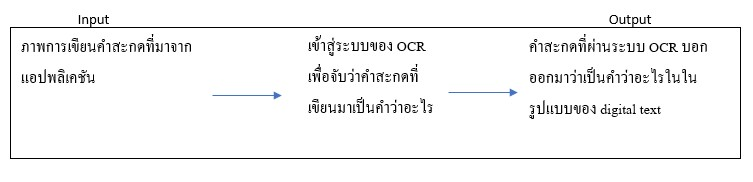
\includegraphics[width=12cm]{./ocrบท3.jpg}}
    \caption{แผนภาพแสดงข้อมูลขาเข้าและออกของการหาลำดับตัวอักษรเพื่อทำนายคำสะกด}\label{fig:system}
   \end{figure}
  \begin{table}[!h]\centering
    \caption{แสดงข้อมูลขาเข้าและขาออกของส่วนการวินิจฉัยการหาลำดับตัวอักษรเพื่อทำนายคำสะกด}\label{tbl:application1}
    \begin{tabular}{c|c|l|rr} \hline
    Input & ภาพการเขียนคำสะกดที่มาจากแอปพลิเคชัน  \\ \hline
    Output & คำสะกดที่ผ่านระบบ OCR บอกออกมาว่าเป็นคำว่าอะไรในในรูปแบบของ digital text \\ \hline
    \end{tabular}
    \end{table}
\newpage
\section{Conceptual  Design}
\begin{figure}[!ht]\centering
  \setlength{\fboxrule}{0.2mm} % can define this in the preamble
  \setlength{\fboxsep}{1cm}
  \fbox{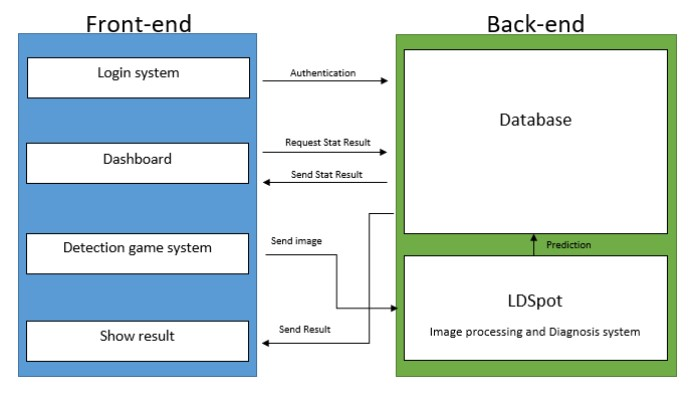
\includegraphics[width=11cm]{./conceptual.jpg}}
  \caption{ภาพการสื่อสารระหว่างทางฝั่ง Frontend และ Backend}\label{fig:conceptual}
 \end{figure}
 การทำงานของตัวระบบ LDSpot นั้นจะมีอยู่สองส่วนด้วยกันได้แก่ front-end ที่ทำหน้าที่เป็นหน้าแอปพลิเคชันไว้สื่อสารกับผู้ใช้งาน และส่วนของ back-end ที่รับข้อมูลมาเพื่อประมวลผลแล้วหลังจากนั้นจึงนำข้อมูลไปเก็บใส่ฐานข้อมูลไว้ใช้งานต่อไป 
 \begin{itemize}
   \item ในส่วนของ front-end นั้นจะประกอบไปด้วย แอปพลิเคชันส์ในรูปแบบของเกม โดยที่ผู้ใช้จะสามารถเข้าสู่ระบบผ่านทางรหัสที่ได้ทำการสมัครสมาชิกไว้
    โดยตัวรหัสจะถูกส่งไปเพื่อตรวจสอบความถูกต้องว่ามีรหัสนี้อยู่จริงในระบบหรือไม่กับฐานข้อมูลที่อยู่ภายในส่วนของ back-end หากตรวจสอบแล้วถูกต้องจึงจะสามารถเข้าสู่ระบบได้ 
   \item ผู้ใช้สามารถกดเข้ารับแบบทดสอบได้ โดยเมื่อเข้ารับแล้ว จะต้องทำตามข้ันตอนต่อไป ซึ่งผู้ใช้จะได้เขียนตัวอักษร สระ และคำสะกด ตามเสียงไปเรื่อยๆ เมื่อเสร็จสิ้นแล้วภาพแบบทดสอบจะถูกส่งไปทางฝั่ง back-end 
   ในส่วนของระบบ LDSpot เพื่อทำการวินิจฉัยหลังจากนั้นผลลัพธ์จะถูกส่งเก็บเข้าไปในฐานข้อมูล เพื่อให้ทางฝั่ง front-end สามารถดึงข้อมูลไปแสดงผลบนแอปพลิเคชันได้
   \item ผู้ใช้สามารถดูผลลัพธ์ย้อนหลังได้โดยกดดูผลลัพธ์ภายในแอปพลิเคชันหลังจากนั้น แอปพลิเคชันจะทำการติดต่อกับฐานข้อมูลเพื่อดึงผลลัพธ์ที่เคยได้มีการวินิจฉัยไว้ของผู้ใช้งานคนนั้นมาแสดงผล
   \item ผู้ใช้สามารถดูบอร์ดสถิติได้ โดยบอร์ดสถิตินั้นจะดึงข้อมูลสรุปจากฐานข้อมูลมาว่า มีผู้ใช้งานแอปพลิเคชันนี้แล้วกี่คน มีการทำนายว่าเป็นโรคบกพร่องทางการเรียนรู้กี่คน ไม่เป็นกี่คนเป็นต้น เพื่อใช้เป็นข้อมูลในเชิงสถิติต่อไป
 \end{itemize}

\begin{landscape}
\section{Database Design}
\begin{figure}[!ht]\centering
    \setlength{\fboxrule}{0.2mm} % can define this in the preamble
    \setlength{\fboxsep}{1cm}
    \fbox{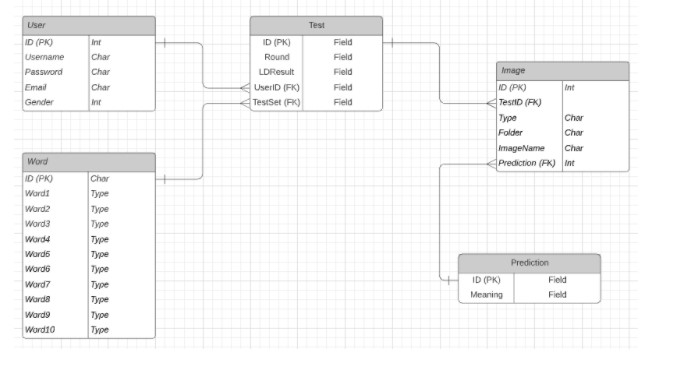
\includegraphics[scale=0.8]{./database.jpg}}
    \caption{ภาพ Database ER diagram}\label{fig:database}
   \end{figure}
  \end{landscape}

\newpage
\section{Sequence Diagram Design}
   \begin{itemize}
    \item ทำแบบทดสอบ 
    Sequence diagram นี้อธิบายขั้นตอนการทำแบบทดสอบโดยในขั้นต้นผู้ทดสอบจะต้องเข้าสู่ระบบผ่านทางแอปพลิเคชันจากนั้นกดเริ่มทำแบบทดสอบทุกครั้งที่มีการเขียนตัวอักษร สระ หรือคำสะกดลงไปแล้วส่งคำตอบ ภาพจะถูกส่งไปที่เซิฟเวอร์ผ่านทาง Django และนำภาพนั้นไปเข้าสู่โมเดลทำนายว่าภาพนั้นเขียนถูกผิด หรือกลับด้านหรือไม่ จากนั้นนำผลลัพธ์ไปเก็บในฐานข้อมูล เพื่อที่ท้ายที่สุดหลังจบแบบทดสอบแล้ว จะสามารถนำผลลัพธ์มาสรุปดูได้ว่า มีการเขียนถูกผิดกลับด้านกี่ตัวและมีโอกาสเป็นโรคบกพร่องทางกราเรียนรู้เท่าใด 
    \begin{figure}[!ht]\centering
      \setlength{\fboxrule}{0.2mm} % can define this in the preamble
      \setlength{\fboxsep}{1cm}
      \fbox{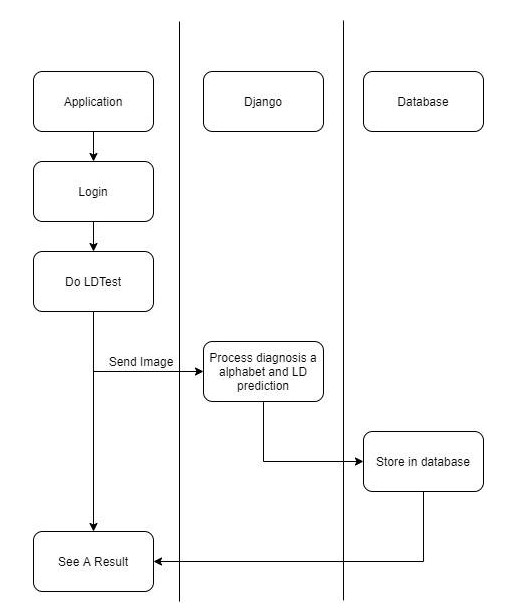
\includegraphics[width=10cm]{./activitytest.jpg}}
      \caption{ภาพ Sequence diagram การทำแบบทดสอบ}\label{fig:activity1}
     \end{figure}
     \newpage
     \begin{table}[!h]\centering
      \caption{Use case narrative ของการทำแบบทดสอบ}\label{tbl:application1}
      \begin{tabular}{|p{4cm}|p{10cm}|} \hline
      Use Case Name & การทำแบบทดสอบ \\ \hline
      Goal in Context & เพื่อให้ได้ภาพตัวอักษร สระ และคำสะกดด้วยลายมือเด็ก \\ \hline
      Primary Actor & ผู้เข้ารับการทำแบบทดสอบ \\ \hline
      Secondary Actor & บุคลากรทางการแพทย์ \\ \hline
      Precondition & ต้องเข้าสู่ระบบก่อน \\ \hline
      Trigger & บุคลากรย์ทางการแพทย์ต้องกรอกชื่อผู้เข้ารับการทดสอบแล้วกดเริ่มการทดสอบ \\ \hline
      Scenario & \begin{enumerate}
        \item บุคลากรย์ทางการแพทย์กดเข้าสู่หน้าเข้ารับการทดสอบ
        \item บุคลากรย์ทางการแพทย์กรอกรหัส ชื่อ นามสกุล ของผู้เข้ารับแบบทดสอบ
        \item ผู้เข้ารับแบบทดสอบเริ่มทำแบบทดสอบการเขียนตัวอักษร สระ และคำสะกดตามลำดับ
        \item ระบบรับภาพตัวอักษร สระ และคำสะกดของผู้รับการทดสอบไปประมวลผลหลังจากนั้นเก็บข้อมูลลงในฐานข้อมูล
        \item บุคลากรย์ทางการแพทย์ สามารถเข้ามาดูผลลัพธ์ได้ในภายหลัง
      \end{enumerate} \\ \hline
      Exception & - \\ \hline
      Post-condition & กดเข้าสู่ระบบดูผลลัพธ์เพื่อดูผลลัพธ์การทดสอบ\\ \hline
      
      \end{tabular}
      \end{table}
    \newpage
    \item ดูผลลัพธ์การทดสอบ
    Sequence diagram นี้อธิบายขั้นตอนการดูผลลัพธ์การทดสอบของผู้ทดสอบโดยจะต้องทำการเข้าสู่ระบบผ่านทางแอปพลิเคชันจากนั้นเข้าส่วนของการดูผลลัพธ์ หลังจากนั้นแอปพลิเคชันจะทำการไปเรียกข้อมูลจากฐานข้อมูลโดยผ่าน Django แล้วนำรายชื่อผลลัพธ์มาแสดงผลผ่านทางแอปพลิเคชัน จากนั้นผู้ทดสอบจะทำการเลือกแบบทดสอบที่ต้องการดูผลลัพธ์ โดยตัวแอปพลิเคชันก็จะดึงข้อมูลจากทางฐานข้อมูลผ่าน Django และนำข้อมูลของผลลัพธ์แบบทดสอบที่ผู้ทดสอบสนใจมาแสดงผลบนแอปพลิเคชัน
    \begin{figure}[!ht]\centering
      \setlength{\fboxrule}{0.2mm} % can define this in the preamble
      \setlength{\fboxsep}{1cm}
      \fbox{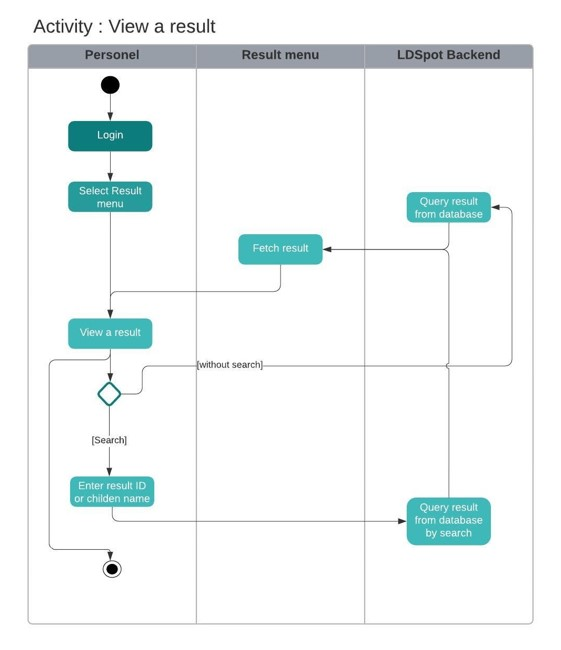
\includegraphics[width=10cm]{./activityresult.jpg}}
      \caption{ภาพ Sequence diagram การดูผลลัพธ์การทดสอบ}\label{fig:activity2}
     \end{figure}
     \newpage
     \begin{table}[!h]\centering
      \caption{Use case narrative ของการดูผลลัพธ์การทดสอบ}\label{tbl:application1}
      \begin{tabular}{|p{4cm}|p{10cm}|} \hline
      Use Case Name & ผลลัพธ์การทดสอบ \\ \hline
      Goal in Context & เพื่อดูผลลัพธ์การทดสอบของผู้เข้ารับการทดสอบ \\ \hline
      Primary Actor & บุคลากรทางการแพทย์\\ \hline
      Secondary Actor & - \\ \hline
      Precondition & ต้องเข้าสู่ระบบก่อน \\ \hline
      Trigger & บุคลากรย์ทางการแพทย์กดเข้าสู่ระบบดูผลลัพธ์ \\ \hline
      Scenario & \begin{enumerate}
        \item บุคลากรย์ทางการแพทย์กดเข้าสู่ระบบดูผลลัพธ์
        \item ระบบดึงรายชื่อแบบทดสอบมาแสดง
        \item บุคลากรย์ทางการแพทย์เลือกแบบทดสอบที่ต้องการจะดูผลลัพธ์
        \item ระบบดึงข้อมูลผลลัพธ์แบบทดสอบนั้นมาแสดง
      \end{enumerate} \\ \hline
      Exception & - \\ \hline
      Post-condition & - \\ \hline
      \end{tabular}
      \end{table}
     \newpage
    \item ดูสถิติรวมของแอปพลิเคชัน
    Sequence diagram นี้อธิบายขั้นตอนการดูสถิติของแอปพลิเคชันโดยผู้ทดสอบจะต้องเข้าสู่ระบบผ่านทางแอปพลิเคชัน จากนั้นเข้าส่วนของการดูสถิติ แอปพลิเคชันจะทำการดึงข้อมูลสรุปผลต่างๆจากฐานข้อมูลเช่น ตัวอักษรใดที่คนเขียนผิดมากที่สุด จำนวนคนใช้แอปพลิเคชันเป็นต้นมาแสดงบนแอปพลิเคชัน
    \begin{figure}[!ht]\centering
      \setlength{\fboxrule}{0.2mm} % can define this in the preamble
      \setlength{\fboxsep}{1cm}
      \fbox{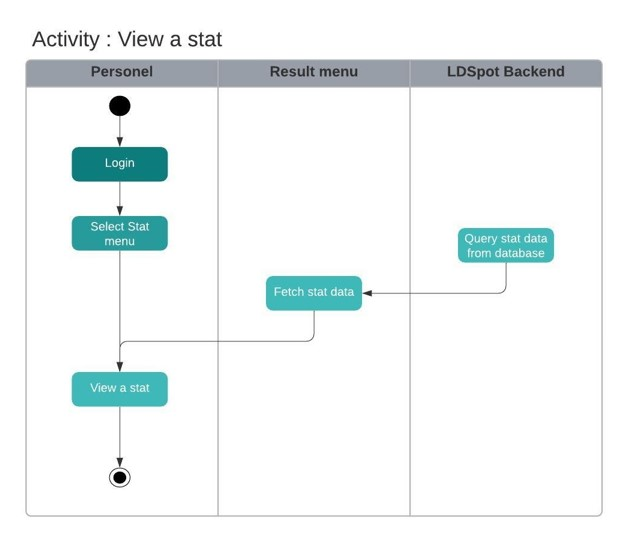
\includegraphics[width=10cm]{./activitystat.jpg}}
      \caption{ภาพ Sequence diagram การดูข้อมูลสถิติในแอปพลิเคชัน}\label{fig:activity3}
     \end{figure}
     \newpage
     \begin{table}[!h]\centering
      \caption{Use case narrative ของการดูข้อมูลสถิติในแอปพลิเคชัน}\label{tbl:application1}
      \begin{tabular}{|p{4cm}|p{10cm}|} \hline
      Use Case Name & ดูข้อมูลสถิติในแอปพลิเคชัน \\ \hline
      Goal in Context & เพื่อดูผลสรุปสถิติของแอปพลิเคชัน \\ \hline
      Primary Actor & บุคลากรทางการแพทย์ \\ \hline
      Secondary Actor & - \\ \hline
      Precondition & ต้องเข้าสู่ระบบก่อน \\ \hline
      Trigger & บุคลากรทางการแพทย์ต้องเข้าสู่หน้าดูสถิติในแอปพลิเคชัน \\ \hline
      Scenario & \begin{enumerate}
        \item บุคลากรทางการแพทย์ต้องเข้าสู่หน้าดูสถิติในแอปพลิเคชัน
        \item ระบบดึงข้อมูลสถิติมาสรุปบนแอปพลิเคชัน
      \end{enumerate} \\ \hline
      Exception & - \\ \hline
      Post-condition & - \\ \hline
  
      \end{tabular}
      \end{table}
  \end{itemize}

\newpage
\section{User Interface Design}
\begin{itemize}
  \item หน้าต่างเข้าสู่ระบบ
  \begin{figure}[!ht]\centering
    \setlength{\fboxrule}{0.2mm} % can define this in the preamble
    \setlength{\fboxsep}{1cm}
    \fbox{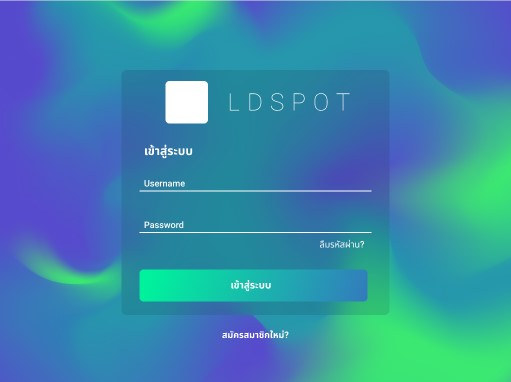
\includegraphics[width=10cm]{./login.jpg}}
    \caption{ภาพการออกแบบหน้าเข้าสู่ระบบ}\label{fig:system}
  \end{figure}
  \item หน้ากรอกข้อมูลสำหรับเริ่มทำแบบทดสอบ
  \begin{figure}[!ht]\centering
    \setlength{\fboxrule}{0.2mm} % can define this in the preamble
    \setlength{\fboxsep}{1cm}
    \fbox{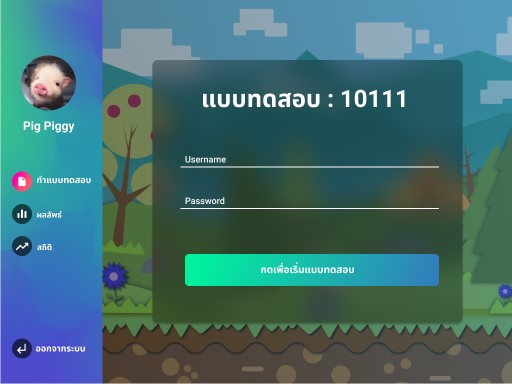
\includegraphics[width=10cm]{./home.jpg}}
    \caption{ภาพการออกแบบหน้ากรอกข้อมูลสำหรับเริ่มทำแบบทดสอบ}\label{fig:system}
  \end{figure}
  \newpage
  \item หน้าแรกของเกมในการทำแบบทดสอบ
  \begin{figure}[!ht]\centering
    \setlength{\fboxrule}{0.2mm} % can define this in the preamble
    \setlength{\fboxsep}{1cm}
    \fbox{
\includegraphics[width=10cm]{./stage1.jpg}}
    \caption{ภาพการออกแบบหน้าการทำแบบทดสอบด่านแรก}\label{fig:system}
  \end{figure}
  \item หน้าสองของเกมในการทำแบบทดสอบ
  \begin{figure}[!ht]\centering
    \setlength{\fboxrule}{0.2mm} % can define this in the preamble
    \setlength{\fboxsep}{1cm}
    \fbox{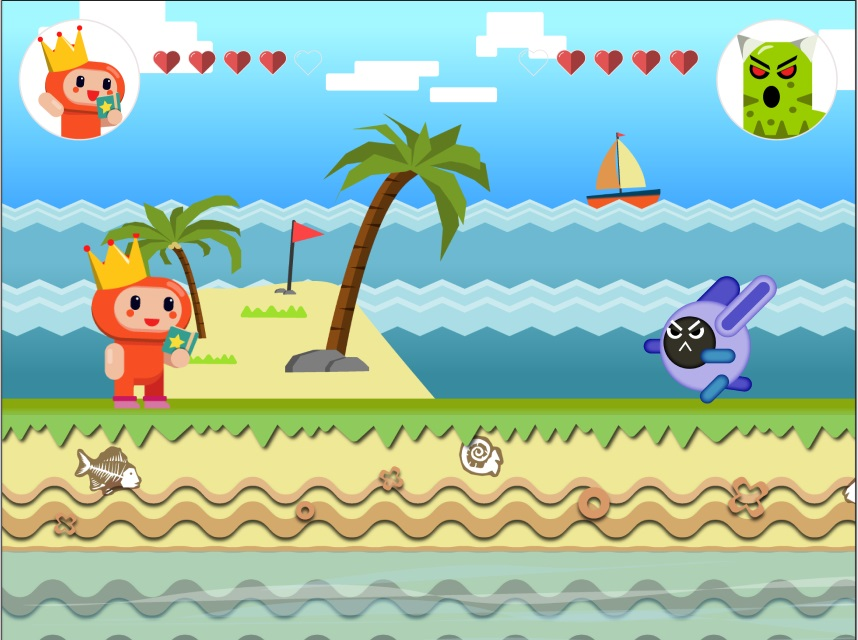
\includegraphics[width=10cm]{./stage2.jpg}}
    \caption{ภาพการออกแบบหน้าการทำแบบทดสอบด่านสอง}\label{fig:system}
  \end{figure}
  \newpage
  \item หน้าสุดท้ายของเกมในการทำแบบทดสอบ
  \begin{figure}[!ht]\centering
    \setlength{\fboxrule}{0.2mm} % can define this in the preamble
    \setlength{\fboxsep}{1cm}
    \fbox{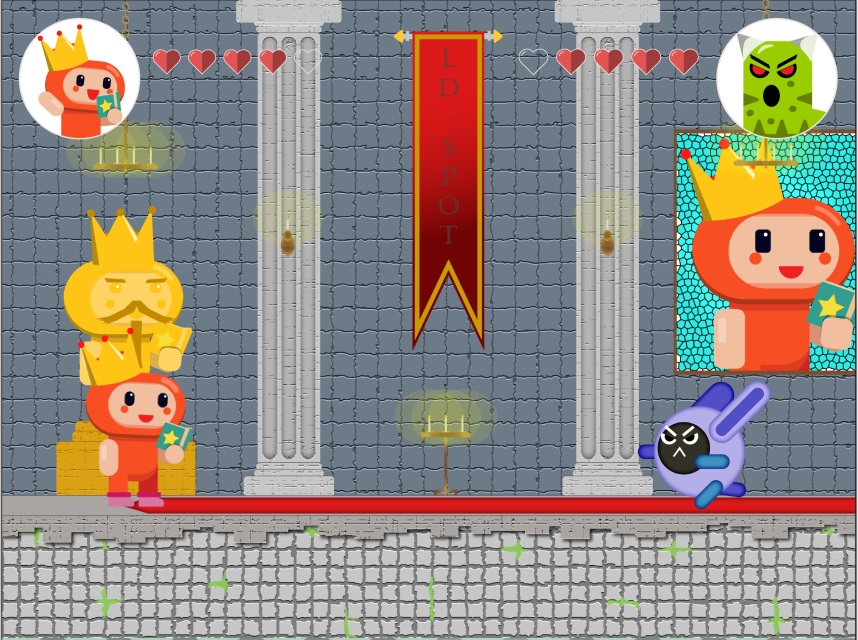
\includegraphics[width=10cm]{./stage3.jpg}}
    \caption{ภาพการออกแบบหน้าการทำแบบทดสอบด่านสาม}\label{fig:system}
  \end{figure}
  \item หน้าปุ่มกดข้ามตัวอักษร สระ หรือคำสะกด
  \begin{figure}[!ht]\centering
    \setlength{\fboxrule}{0.2mm} % can define this in the preamble
    \setlength{\fboxsep}{1cm}
    \fbox{
\includegraphics[width=10cm]{./stage1inputSkip.jpg}}
    \caption{ภาพการออกแบบหน้าการกดข้ามการเขียนตัวอักษร สระ และคำสะกด}\label{fig:system}
  \end{figure}
  \newpage
  \item หน้าต่างสำหรับเขียนตัวอักษร สระ และคำสะกด
  \begin{figure}[!ht]\centering
    \setlength{\fboxrule}{0.2mm} % can define this in the preamble
    \setlength{\fboxsep}{1cm}
    \fbox{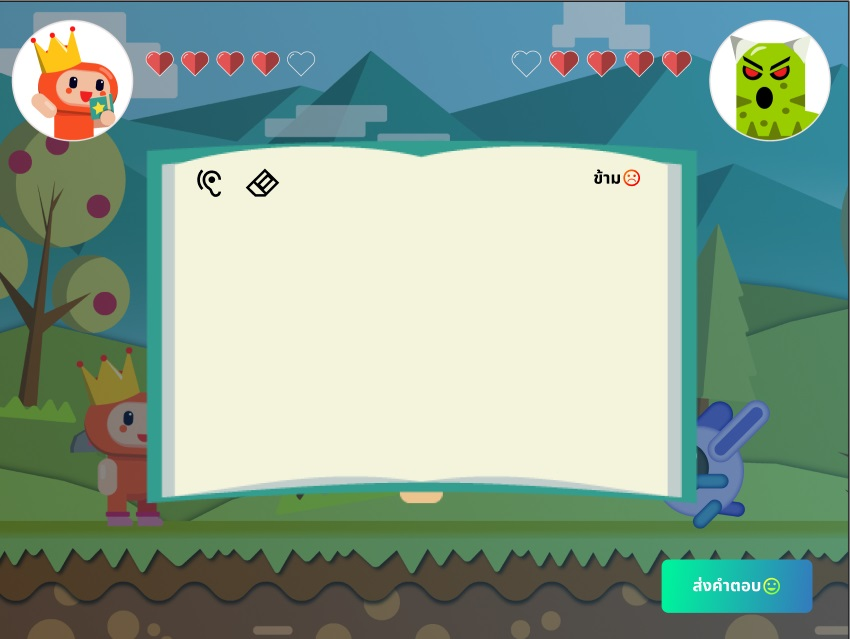
\includegraphics[width=10cm]{./stage1input.jpg}}
    \caption{ภาพการออกแบบหน้าเขียนตัวอักษร สระ และคำสะกด}\label{fig:system}
  \end{figure}
  \begin{figure}[!ht]\centering
    \setlength{\fboxrule}{0.2mm} % can define this in the preamble
    \setlength{\fboxsep}{1cm}
    \fbox{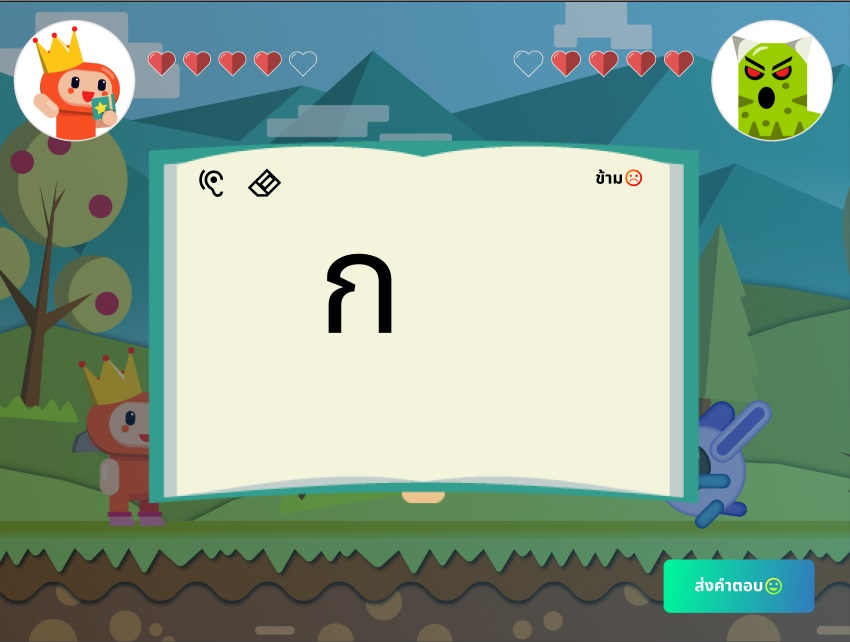
\includegraphics[width=10cm]{./stage1input2.jpg}}
    \caption{ภาพการออกแบบหน้าเขียนตัวอักษร สระ และคำสะกด}\label{fig:system}
  \end{figure}
  \newpage
  \item หน้าเกมสำหรับจบแบบทดสอบ
  \begin{figure}[!ht]\centering
    \setlength{\fboxrule}{0.2mm} % can define this in the preamble
    \setlength{\fboxsep}{1cm}
    \fbox{
\includegraphics[width=10cm]{./endGame.jpg}}
    \caption{ภาพการออกแบบหน้าจบการทดสอบ}\label{fig:system}
  \end{figure}s
  \item หน้าดูผลลัพธ์การทดสอบ
    \begin{figure}[!ht]\centering
      \setlength{\fboxrule}{0.2mm} % can define this in the preamble
      \setlength{\fboxsep}{1cm}
      \fbox{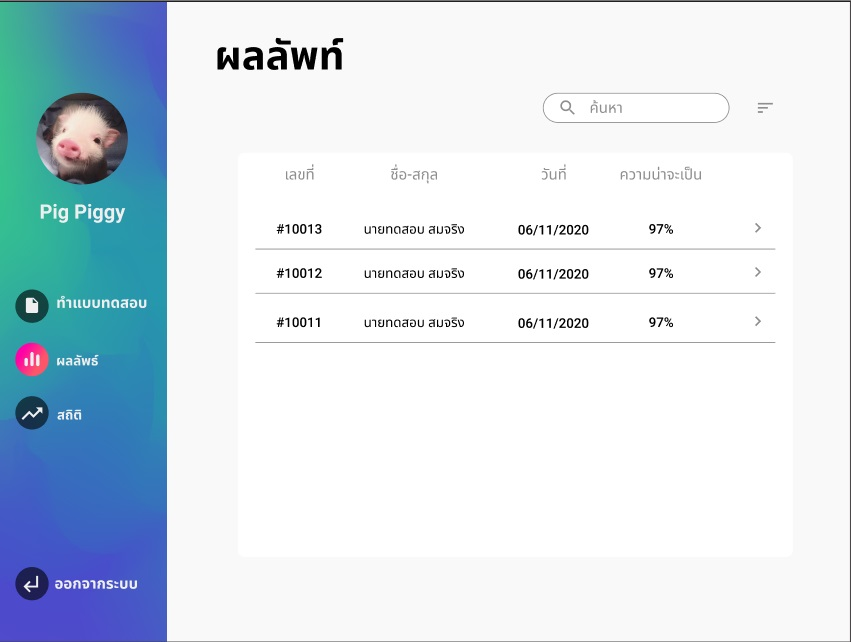
\includegraphics[width=10cm]{./result.jpg}}
      \caption{ภาพออกแบบหน้าดูผลลัพธ์การทดสอบ}\label{fig:system}
    \end{figure}
  \newpage
  \item หน้าดูข้อมูลสถิติภายในแอปพลิเคชัน
    \begin{figure}[!ht]\centering
      \setlength{\fboxrule}{0.2mm} % can define this in the preamble
      \setlength{\fboxsep}{1cm}
      \fbox{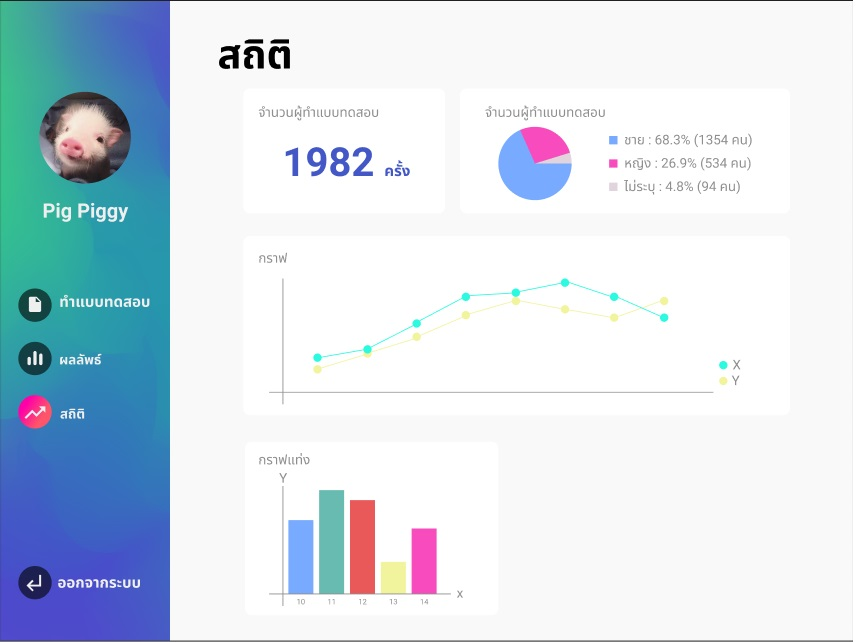
\includegraphics[width=10cm]{./stat.jpg}}
      \caption{ภาพการออกแบบหน้าดูสถิติภายในแอปพลิเคชัน}\label{fig:system}
        
  \end{figure}
\end{itemize}
\newpage
\section{การเก็บข้อมูลภาพลายมือเด็ก}
การเก็บรวมรวมข้อมูลของภาพลายมือเด็ก เราได้ทำการรวมรวมรูปภาพการทำแบบทดสอบโดยเขียนพยัญชนะ สระ และคำสะกด 
จากนักเรียนระดับชั้นประถมศึกษาตั้งแต่ประถมศึกษาปีที่หนึ่งถึงประถมศึกษาปีที่สาม โดยคาดว่าจะมีเด็กเข้าร่วมทำแบบทดสอบประมาณ 1000 
คนโดยประมาณ ซึ่งภาพลายมือเด็กที่เขียนถูกต้องจะถูกนำมาใช้ในการเรียนรู้ของตัวโมเดลของเรา โดยตัวอย่างแบบทดสอบมีดังนี้
\begin{figure}[!ht]\centering
  \setlength{\fboxrule}{0.2mm} % can define this in the preamble
  \setlength{\fboxsep}{1cm}
  \fbox{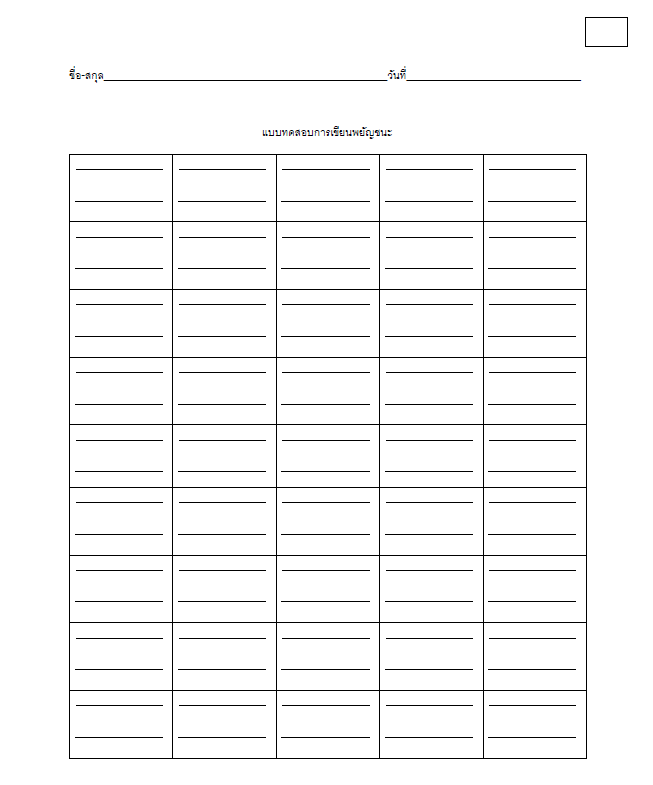
\includegraphics[width=10cm,height=10cm]{./พยัญชนะ.png}}
  \caption{ภาพแบบทดสอบที่ใช้เก็บลายมือตัวอักษรเด็ก}\label{fig:system}
    
\end{figure}
\newpage
\begin{figure}[!ht]\centering
  \setlength{\fboxrule}{0.2mm} % can define this in the preamble
  \setlength{\fboxsep}{1cm}
  \fbox{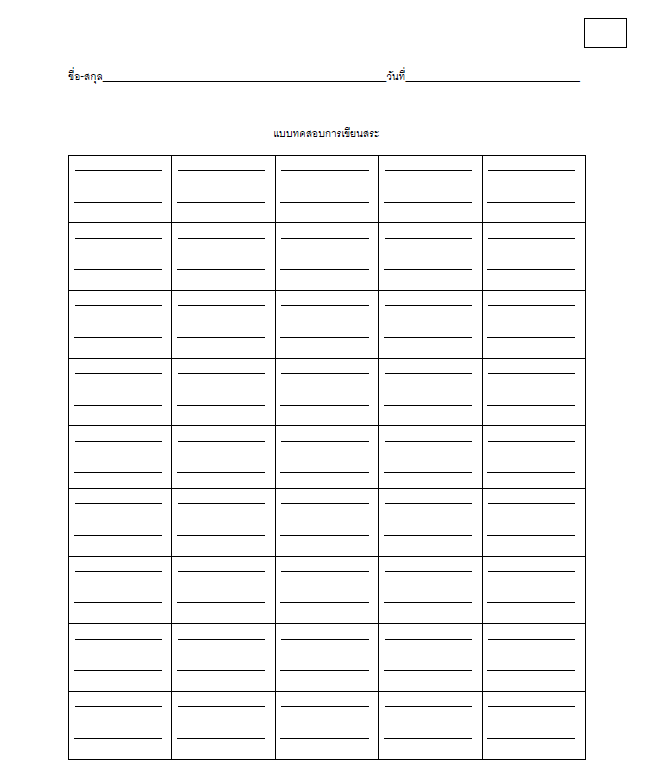
\includegraphics[width=10cm,height=10cm]{./สระ.png}}
  \caption{ภาพแบบทดสอบที่ใช้เก็บลายมือสระเด็ก}\label{fig:system}
    
\end{figure}
\begin{figure}[!ht]\centering
  \setlength{\fboxrule}{0.2mm} % can define this in the preamble
  \setlength{\fboxsep}{1cm}
  \fbox{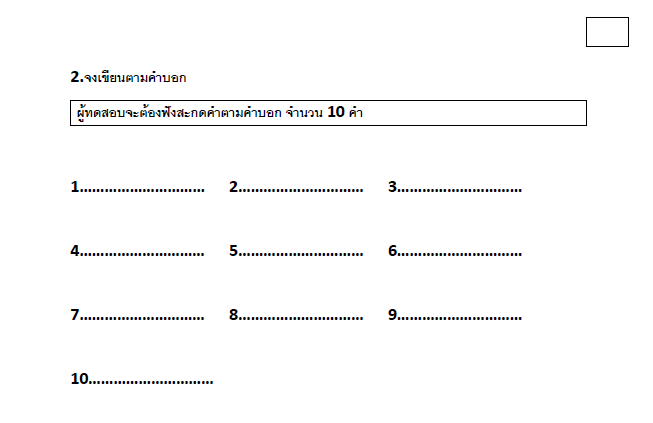
\includegraphics[width=10cm]{./คำสะกด.png}}
  \caption{ภาพแบบทดสอบที่ใช้เก็บลายมือคำสะกดเด็ก}\label{fig:system}
    
\end{figure}

\newpage
\section{แผนการประเมินประสิทธิภาพของแอปพลิเคชัน}
เราจะนำตัวแอปพลิเคชันไปวัดผลที่ หน่วยตรวจโรคจิตเวชเด็กและวัยรุ่น ภาควิชาจิตเวชศาสตร์ คณะแพทยศาสตร์ศิริราชพยาบาล  ซึ่งบุคลากรจะนำตัวแอปพลิเคชันไปทดสอบกับเด็ก เพื่อสังเกตผลลัพธ์ว่า แอปพลิเคชันกับบุคลากรนั้น สามารถจำแนกประเภทอาการของเด็กออกมาได้ตรงกันหรือไม่ 
\subsection{การวัดผลความแม่นยำของระบบ LDSpot}
สามารถวัดผลได้โดยการใช้ Confusion matrix 

\begin{table}[!h]\centering
  \caption{ตาราง Confusion Matrix}\label{tbl:confusion}
  \begin{tabular}{c|c|l|rr} \hline
  ตารางการวินิจฉัย & Actual Positive & Actual Negative \\ \hline
  Predict Positive & & \\ \hline
  Predict Negative & & \\ \hline
  \end{tabular}
  \end{table}


แบบสอบถามประเมินความพึงพอใจจากบุคลากรทางการแพทย์

\chapter{ผลการดำเนินงาน}
\section{Application}
ตัวอย่างแอปพลิเคชันที่ดำเนินการสร้างเสร็จ
\begin{itemize}
  \item  หน้าแรกของเกมที่ใช้ทำแบบทดสอบ  
  \begin{figure}[!h]\centering
    \setlength{\fboxrule}{0.2mm} % can define this in the preamble
    \setlength{\fboxsep}{1cm}
    \fbox{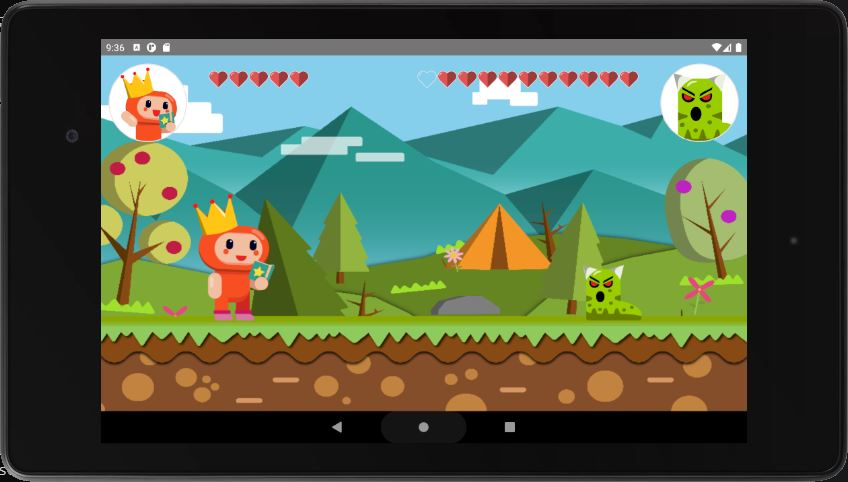
\includegraphics[width=10cm]{./gamesceneหน้ารอเขียน.JPG}}
    \caption{ภาพหน้าจอแอปพลิเคชันแบบทดสอบ}\label{fig:system}
  \end{figure}
    \item  หน้าต่างสำหรับการเขียนตัวอักษร สระ และคำสะกดสำหรับแบบทดสอบ
     \begin{figure}[!h]\centering
      \setlength{\fboxrule}{0.2mm} % can define this in the preamble
      \setlength{\fboxsep}{1cm}
      \fbox{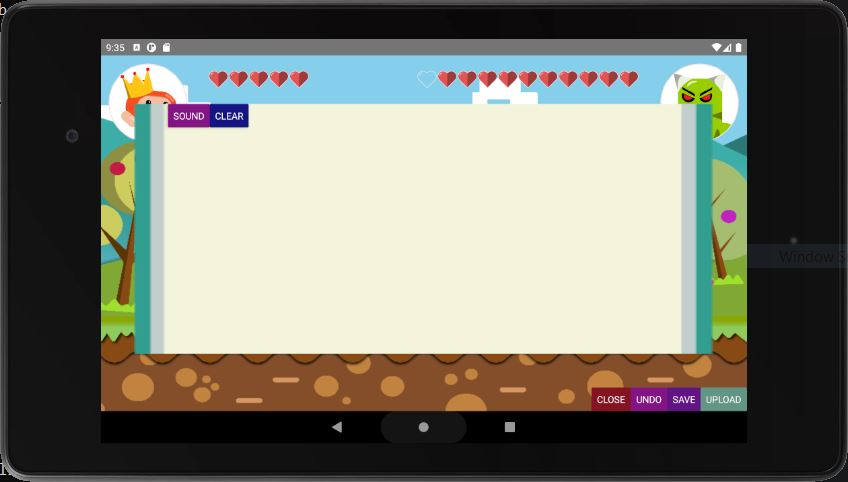
\includegraphics[width=10cm]{./gamesceneหน้าต่างเขียน.JPG}}
      \caption{ภาพหน้าจอแอปพลิเคชันแบบทดสอบสำหรับเขียน}\label{fig:system}
    \end{figure}
  \newpage
 \item  หน้าต่างสำหรับการเขียนตัวอักษร สระ และคำสะกดสำหรับแบบทดสอบ
  \begin{figure}[!h]\centering
    \setlength{\fboxrule}{0.2mm} % can define this in the preamble
    \setlength{\fboxsep}{1cm}
    \fbox{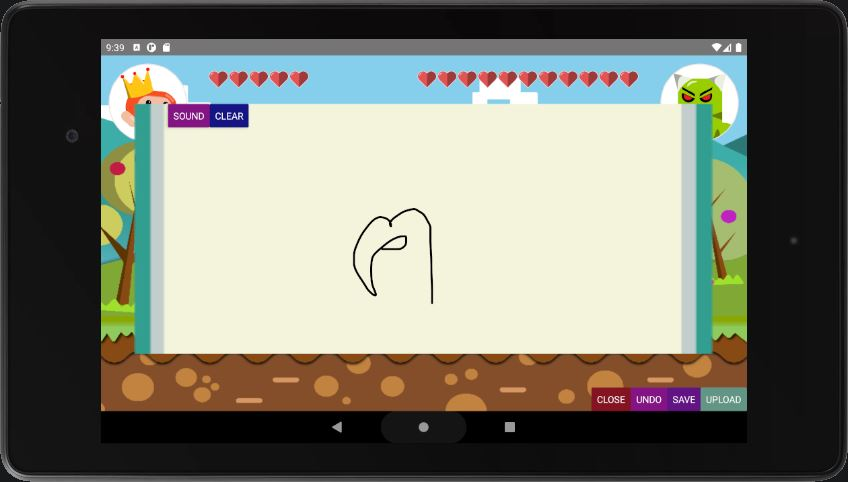
\includegraphics[width=10cm]{./gamesceneหน้าต่างเขียนแล้ว.JPG}}
    \caption{ภาพหน้าจอแอปพลิเคชันแบบทดสอบสำหรับเขียน}\label{fig:system}
  \end{figure}
 \item   ตัวอย่างการเล่นปล่อยพลังภายในเกม
 \begin{figure}[!h]\centering
    \setlength{\fboxrule}{0.2mm} % can define this in the preamble
    \setlength{\fboxsep}{1cm}
    \fbox{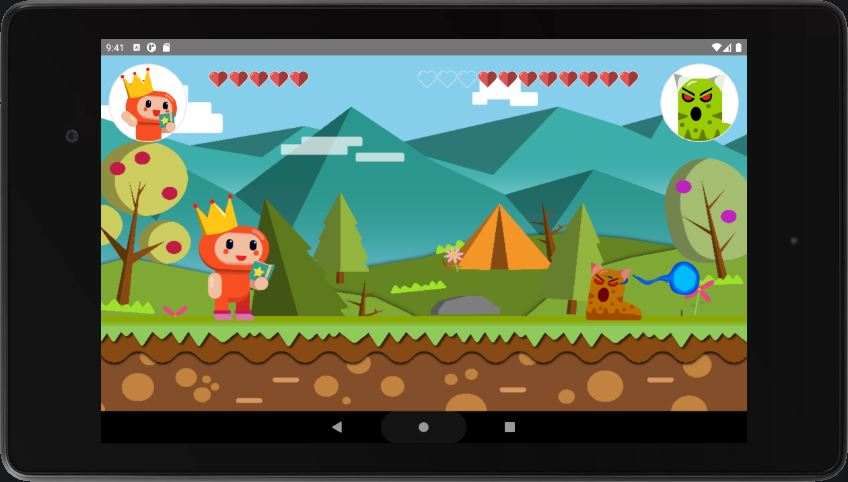
\includegraphics[width=10cm]{./gamesceneปล่อยท่า.JPG}}
    \caption{ภาพหน้าจอแอปพลิเคชันการปล่อยพลัง}\label{fig:system}
  \end{figure}       
  \newpage   
 \item หน้าจบด่านแรกของเกมที่ใช้ในการทำแบบทดสอบ
 \begin{figure}[!h]\centering
    \setlength{\fboxrule}{0.2mm} % can define this in the preamble
    \setlength{\fboxsep}{1cm}
    \fbox{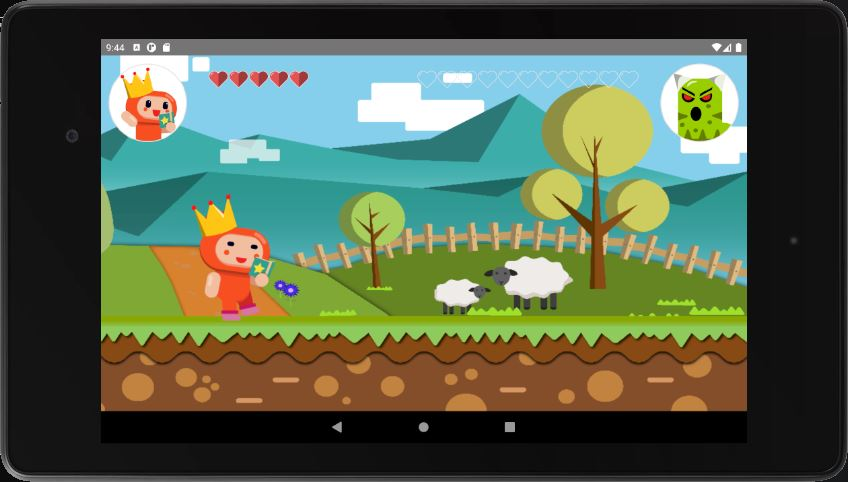
\includegraphics[width=10cm]{./gamesceneจบฉากแรก.JPG}}
    \caption{ภาพหน้าจอแอปพลิเคชันหน้าจบด่านแรก}\label{fig:system}
  \end{figure}
 \item หน้าดูผลลัพธ์แบบทดสอบของเด็กทั้งหมด 
  \begin{figure}[!h]\centering
    \setlength{\fboxrule}{0.2mm} % can define this in the preamble
    \setlength{\fboxsep}{1cm}
    \fbox{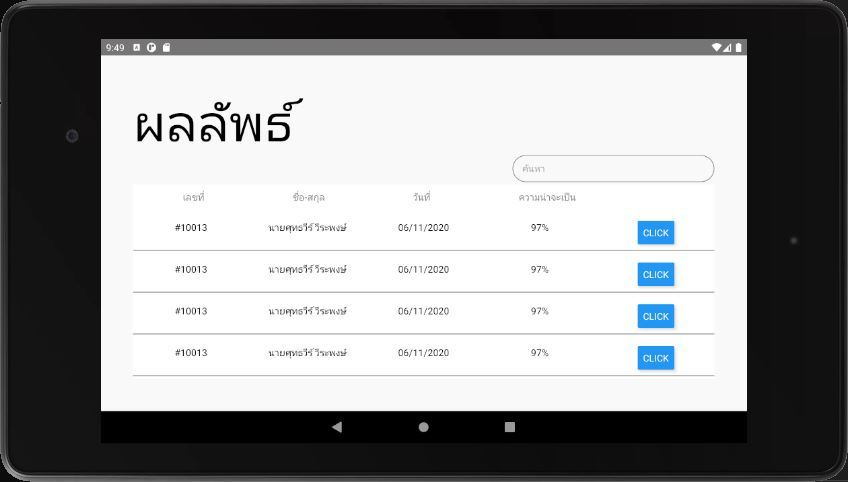
\includegraphics[width=10cm]{./statหน้ารวม.JPG}}
    \caption{ภาพหน้าจอแอปพลิเคชันดูผลลัพธ์}\label{fig:system}
  \end{figure}
  \newpage
 \item หน้าดูผลลัพธ์แบบทดสอบของเด็กภายใน
  \begin{figure}[!h]\centering
    \setlength{\fboxrule}{0.2mm} % can define this in the preamble
    \setlength{\fboxsep}{1cm}
    \fbox{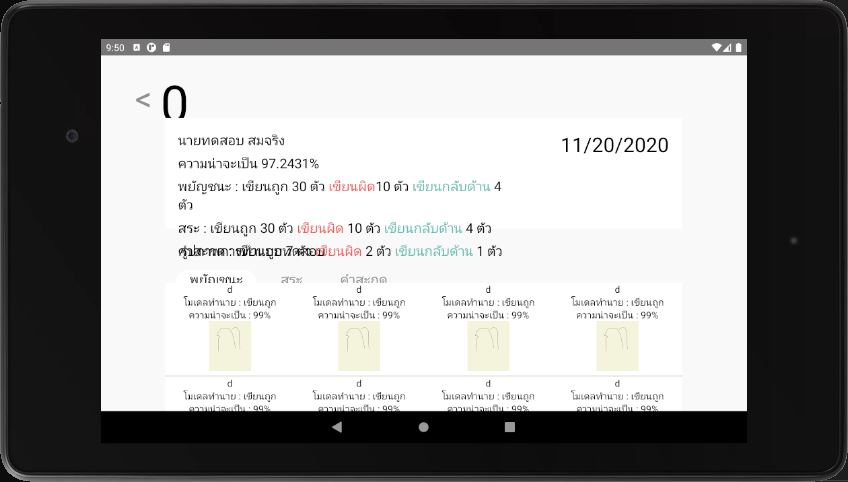
\includegraphics[width=10cm]{./statหน้าย่อย.JPG}}
    \caption{ภาพหน้าจอแอปพลิเคชันดูผลลัพธ์รายคน}\label{fig:system}
  \end{figure}
 \item ภาพแบบทดสอบของเด็ก
  \begin{figure}[!h]\centering
    \setlength{\fboxrule}{0.2mm} % can define this in the preamble
    \setlength{\fboxsep}{1cm}
    \fbox{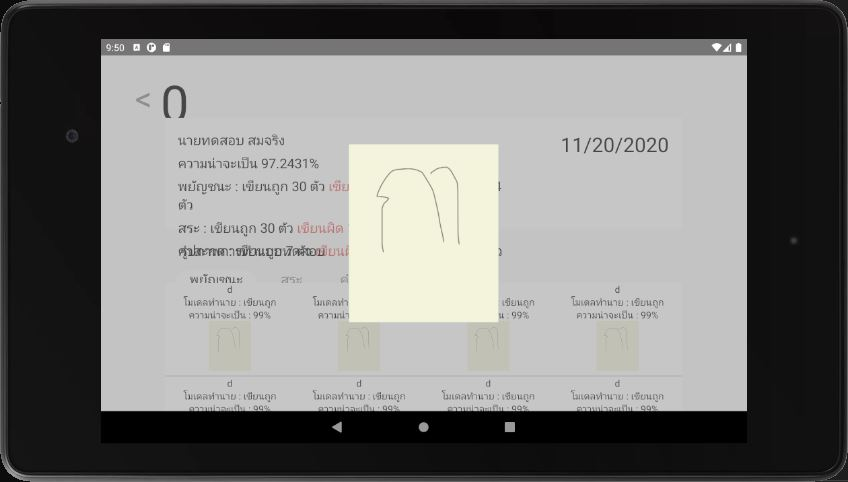
\includegraphics[width=10cm]{./statหน้ารวมดูรูป.JPG}}
    \caption{ภาพหน้าจอแอปพลิเคชันดูผลลัพธ์การทดสอบ}\label{fig:system}                  
   \end{figure}
\end{itemize}
\newpage
\section{OCR }
  OCR ที่นำมาใช้คู่กับโมเดลทำนายตัวอักษรเพื่อที่จะวิเคราะห์ว่าคำสะกดที่ผู้ทำแบบทดสอบเขียนมาถูกต้องหรือไม่ โดยในส่วนของความแม่นยำของ OCR นั้นจากการทดสอบนำรูปภาพลายมือเขียนจำนวน 111 ตัวอักษรมาทดสอบพบว่า สามารถแยกตัวอักษรได้ถูกต้องเป็นจำนวน 96 ภาพ คิดเป็น 87\% จากทั้งหมด
\begin{itemize}
  \item ภาพตัวอักษร
  \begin{figure}[!h]\centering
    \setlength{\fboxrule}{0.2mm} % can define this in the preamble
    \setlength{\fboxsep}{1cm}
    \fbox{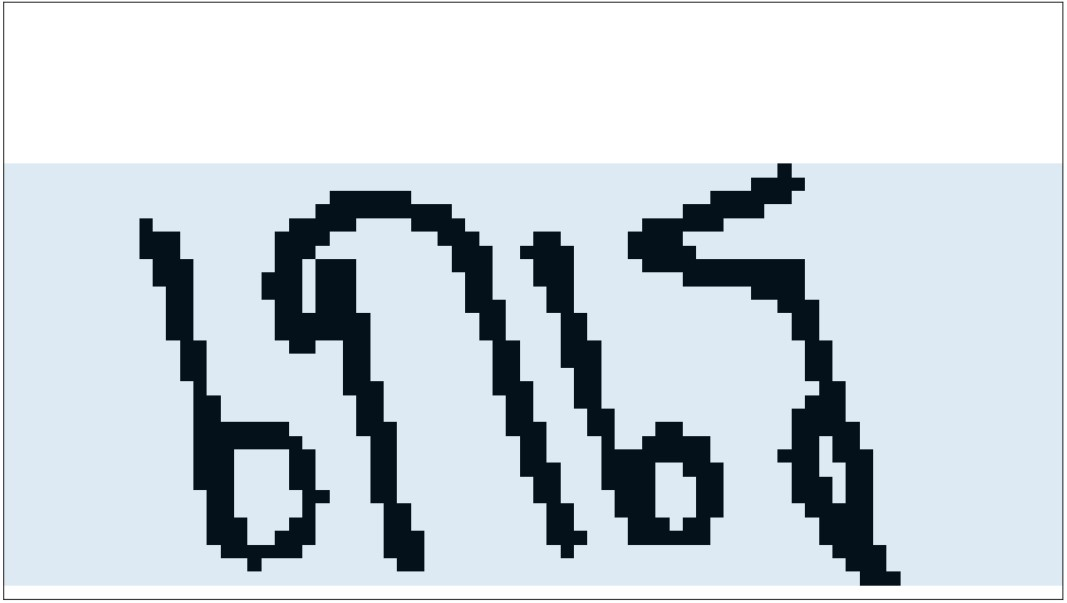
\includegraphics[width=10cm]{ocrpython.jpg}}
    \caption{ภาพลายมือเขียนของเด็ก}\label{fig:system}                  
   \end{figure}
   \item ภาพตัวอักษรหลังผ่านการทำ bounding box แล้ว
   \begin{figure}[!h]\centering
     \setlength{\fboxrule}{0.2mm} % can define this in the preamble
     \setlength{\fboxsep}{1cm}
     \fbox{\includegraphics[width=10cm]{ocrpython2.jpg}}
     \caption{ภาพลายมือเขียนของเด็กที่ได้ทำการแบ่งตัวอักษรแล้ว}\label{fig:system}                  
    \end{figure}
    \newpage
    \item ภาพตัวอักษร
  \begin{figure}[!h]\centering
    \setlength{\fboxrule}{0.2mm} % can define this in the preamble
    \setlength{\fboxsep}{1cm}
    \fbox{\includegraphics[width=10cm]{ocr3.jpg}}
    \caption{ภาพลายมือเขียนของเด็ก}\label{fig:system}                  
   \end{figure}
   \item ภาพ bounding box ที่พบว่ามีตัวอักษรมากกว่าหนึ่งตัว
  \begin{figure}[!h]\centering
    \setlength{\fboxrule}{0.2mm} % can define this in the preamble
    \setlength{\fboxsep}{1cm}
    \fbox{\includegraphics[width=10cm]{ocrpython4.jpg}}
    \caption{ภาพลายมือเขียนของเด็กที่ทำการ bounding box แล้วมีมากกว่า 1 ตัวอักษร}\label{fig:system}                  
   \end{figure}
   \newpage
   \item ภาพตัวอักษรหลังผ่านการทำ bounding box แล้ว
   \begin{figure}[!h]\centering
     \setlength{\fboxrule}{0.2mm} % can define this in the preamble
     \setlength{\fboxsep}{1cm}
     \fbox{\includegraphics[width=10cm]{ocrpython5.jpg}}
     \caption{ภาพหลังการทำ bounding box แล้ว}\label{fig:system}                  
    \end{figure}
\end{itemize}
\section{ ระบบเก็บรวบรวมข้อมูลทดสอบการเขียนของเด็กที่ได้รับบการทดสอบ}
มีการเตรียมระบบสำหรับตัดตัวอักษร สระ และคำสะกดภายในแบบทดสอบที่เด็กเขียนแล้วทำการแบ่งแยกออกมาเป็นประเภทของตัวอักษร สระ และคำสะกดเตรียมไว้สำหรับการสร้างโมเดล Convolutional Neural Network
\begin{figure}[!h]\centering
  \setlength{\fboxrule}{0.2mm} % can define this in the preamble
  \setlength{\fboxsep}{1cm}
  \fbox{\includegraphics[scale=0.3]{prepareinformation.jpg}}
  \caption{ภาพแบบทดสอบของเด็กที่ผ่านการทำ bounding box}\label{fig:system}                  
 \end{figure}
 \newpage
 \begin{figure}[!h]\centering
  \setlength{\fboxrule}{0.2mm} % can define this in the preamble
  \setlength{\fboxsep}{1cm}
  \fbox{\includegraphics[]{exampleimage.jpg}}
  \caption{ภาพตัวอักษรจากแบบทดสอบที่ผ่านการตัดมาเตรียมไว้ใช้สำหรับการสร้างโมเดล Convolutional Neural Network}\label{fig:system}                  
 \end{figure}
\section{ส่วนที่กำลังดำเนินการภายในภาคการศึกษาที่ 1}
ในส่วนของข้อมูลที่ผ่านการประมวลผลที่เตรียมพร้อมสำหรับนำไปสร้างโมเดลในการวิเคราะห์โรคบกพร่องทางการเรียนรู้ และ  โมเดลจำแนกประเภทรูปภาพแบบเบื้องต้นด้วย Convolutional Neural Network
เนื่องจากต้องติดต่อโรงเรียนต่างๆ เพื่อเข้าไปขอเก็บข้อมูลลายมือของเด็ก และต้องทำการขอใบจริยธรรมเนื่องจากตัวงานวิจัยนั้นมีการใช้งานกับมนุษย์ ทำให้ต้องติดต่อกับหลายส่วนแล้วใช้เวลาในการดำเนินการ ทำให้ยังไม่สามารถเตรียมข้อมูลที่ผ่านการประมวลสำหรับไปใช้สร้างโมเดล Convolutional Neural Network ที่ใช้ในการวิเคราะห์ตัวอักษรที่ผู้ทำแบบทดสอบเขียนได้

%%%%%%%%%%%%%%%%%%%%%%%%%%%%%%%%%%%%%%%%%%%%%%%%%%%%%%%%%%%%%%%
%%%%%%%%%%%%%%%%%%%% Bibliography %%%%%%%%%%%%%%%%%%%%%%%%%%%%%
%%%%%%%%%%%%%%%%%%%%%%%%%%%%%%%%%%%%%%%%%%%%%%%%%%%%%%%%%%%%%%%


%%%% Comment this in your report to show only references you have
%%%% cited. Otherwise, all the references below will be shown.
\nocite{*}
%% Use the kmutt.bst for bibtex bibliography style 
%% You must have cpe.bib and string.bib in your current directory.
%% You may go to file .bbl to manually edit the bib items.
\bibliographystyle{kmutt}
\bibliography{string,cpe}



\end{document}
